\section{Analiza wyników dla datasetu \textbf{WELFake}}
\label{subsec:welfake_analysis}

W tej sekcji przedstawiono szczegółową analizę wyników uzyskanych dla datasetu \textbf{WELFake} w trzech trybach uczenia: \textbf{klasycznym}, \textbf{few-shot} oraz \textbf{one-shot}. Analiza obejmuje kluczowe metryki wydajności, takie jak \textbf{Dokładność (Accuracy)}, \textbf{Wynik F1 (F1-Score)} oraz \textbf{Pole pod krzywą ROC-AUC (ROC-AUC)}, dla embeddingów językowych \textbf{BERT}, \textbf{RoBERTa} oraz \textbf{SBERT}. Wyniki przedstawiono w formie histogramów ilustrujących rozkłady metryk oraz wykresów liniowych czasu wykonania eksperymentów. Szczególną uwagę poświęcono metodom autorskim (\texttt{Metoda17}, \texttt{Metoda18}, \texttt{Metoda19}, \texttt{Metoda20}), omawiając przyczyny ich wydajności oraz różnice w skuteczności w zależności od typu embeddingu i trybu uczenia. Wnioski podsumowano w osobnej podsekcji, uwzględniając sens stosowania bardziej złożonych metod w kontekście uzyskanych wyników.

% Subsection for classical mode results
\subsection{Wyniki w trybie klasycznym}

W trybie \textbf{klasycznym} dla datasetu \textbf{WELFake} przetestowano różne metody klasyfikacji, wykorzystując embeddingi \textbf{BERT}, \textbf{RoBERTa} oraz \textbf{SBERT}. Poniżej przedstawiono szczegółowy opis wyników w formie histogramów dla kluczowych metryk oraz wykresu liniowego czasu wykonania eksperymentów, z uwzględnieniem przyczyn zróżnicowania wydajności metod.

\subsubsection{Accuracy}
Wykresy słupkowe \textbf{Dokładności (Accuracy)} \ref{fig:welfake_classic_accuracy} przedstawiają rozkład wartości dokładności dla wszystkich metod. Na podstawie wykresów można sformułować następujące obserwacje:

\begin{itemize}
	\item \textbf{Wykres górny (BERT):}
	      \begin{itemize}
		      \item Najlepsze wyniki, na poziomie około 0.9, osiągnęły metody \texttt{Metoda12-rf} (oparta na Random Forest), \texttt{Metoda14} (model zespołowy stacking z Random Forest, AdaBoost i SVC), \texttt{Metoda16} (stacking z meta-klasyfikatorem opartym na regresji logistycznej) oraz autorska \texttt{Metoda19} (model stackingowy). Wysoka skuteczność tych metod wskazuje na ich zdolność do efektywnego wykorzystywania bogatych i złożonych cech generowanych przez model BERT, co przekłada się na precyzyjną klasyfikację.
		      \item Najgorsze wyniki, na poziomie około 0.6, odnotowano dla autorskiej \texttt{Metoda17} (zaawansowany VotingClassifier). Niska dokładność tej metody może wynikać z nieoptymalnego doboru wag głosowania lub klasyfikatorów bazowych, które nie były w stanie efektywnie przetworzyć złożonych embeddingów BERT w kontekście klasycznej walidacji.
	      \end{itemize}

	\item \textbf{Wykres środkowy (RoBERTa):}
	      \begin{itemize}
		      \item Najlepsze wyniki, na poziomie około 0.95, osiągnęły \texttt{Metoda12-rf}, \texttt{Metoda14} oraz autorska \texttt{Metoda19}. Wysoka skuteczność tych metod sugeruje, że embeddingi RoBERTa są dobrze dopasowane do zaawansowanych technik ensemble, takich jak stacking i Random Forest, umożliwiając efektywne wykorzystanie złożonych wzorców w danych.
		      \item Najgorsze wyniki, około 0.65, odnotowano dla \texttt{Metoda17}. Niska dokładność tej metody, podobnie jak w przypadku BERT, może wskazywać na trudności w generalizacji dla embeddingów RoBERTa z powodu nieoptymalnej konfiguracji VotingClassifiera.
	      \end{itemize}

	\item \textbf{Wykres dolny (SBERT):}
	      \begin{itemize}
		      \item Większość metod, w tym autorskie \texttt{Metoda17}, \texttt{Metoda18} oraz \texttt{Metoda20}, osiągnęła dokładność na poziomie około 0.95. Ten wynik wskazuje, że embeddingi SBERT dostarczają wysoce informatywnych cech, które mogą być efektywnie przetwarzane zarówno przez zaawansowane modele ensemble, jak i prostsze architektury.
		      \item Najgorsze wyniki, około 0.7, odnotowano dla \texttt{Metoda4} (architektura oparta na zespole sieci Bi-LSTM, CNN i MLP). Niska dokładność tej metody może sugerować, że jej złożona struktura nie była odpowiednio zoptymalizowana dla embeddingów SBERT, co skutkuje słabszą zdolnością klasyfikacji.
	      \end{itemize}
\end{itemize}

Analiza wykresów słupkowych dokładności ujawnia, że modele oparte na ensemble learning, takie jak \texttt{Metoda12-rf}, \texttt{Metoda14}, \texttt{Metoda16} oraz \texttt{Metoda19}, osiągają wysoką skuteczność w trybie klasycznym, szczególnie dla BERT i RoBERTa. Autorska \texttt{Metoda19} wyróżnia się jako stabilna i skuteczna dla wszystkich embeddingów, co podkreśla potencjał dobrze skonfigurowanych modeli stackingowych. Z kolei \texttt{Metoda17} wykazuje słabsze wyniki dla BERT i RoBERTa, co może wynikać z nieoptymalnego doboru klasyfikatorów bazowych w VotingClassifierze. \texttt{Metoda18} i \texttt{Metoda20} osiągają dobre wyniki dla SBERT, co wskazuje na ich zdolność do efektywnego wykorzystywania informatywnych cech tego embeddingu. \texttt{Metoda20} osiąga średnie wyniki dla BERT z powodu braku odpowiedniego balansowania klas, co ogranicza jej skuteczność w bardziej złożonych scenariuszach.

\begin{figure}[H]
	\centering
	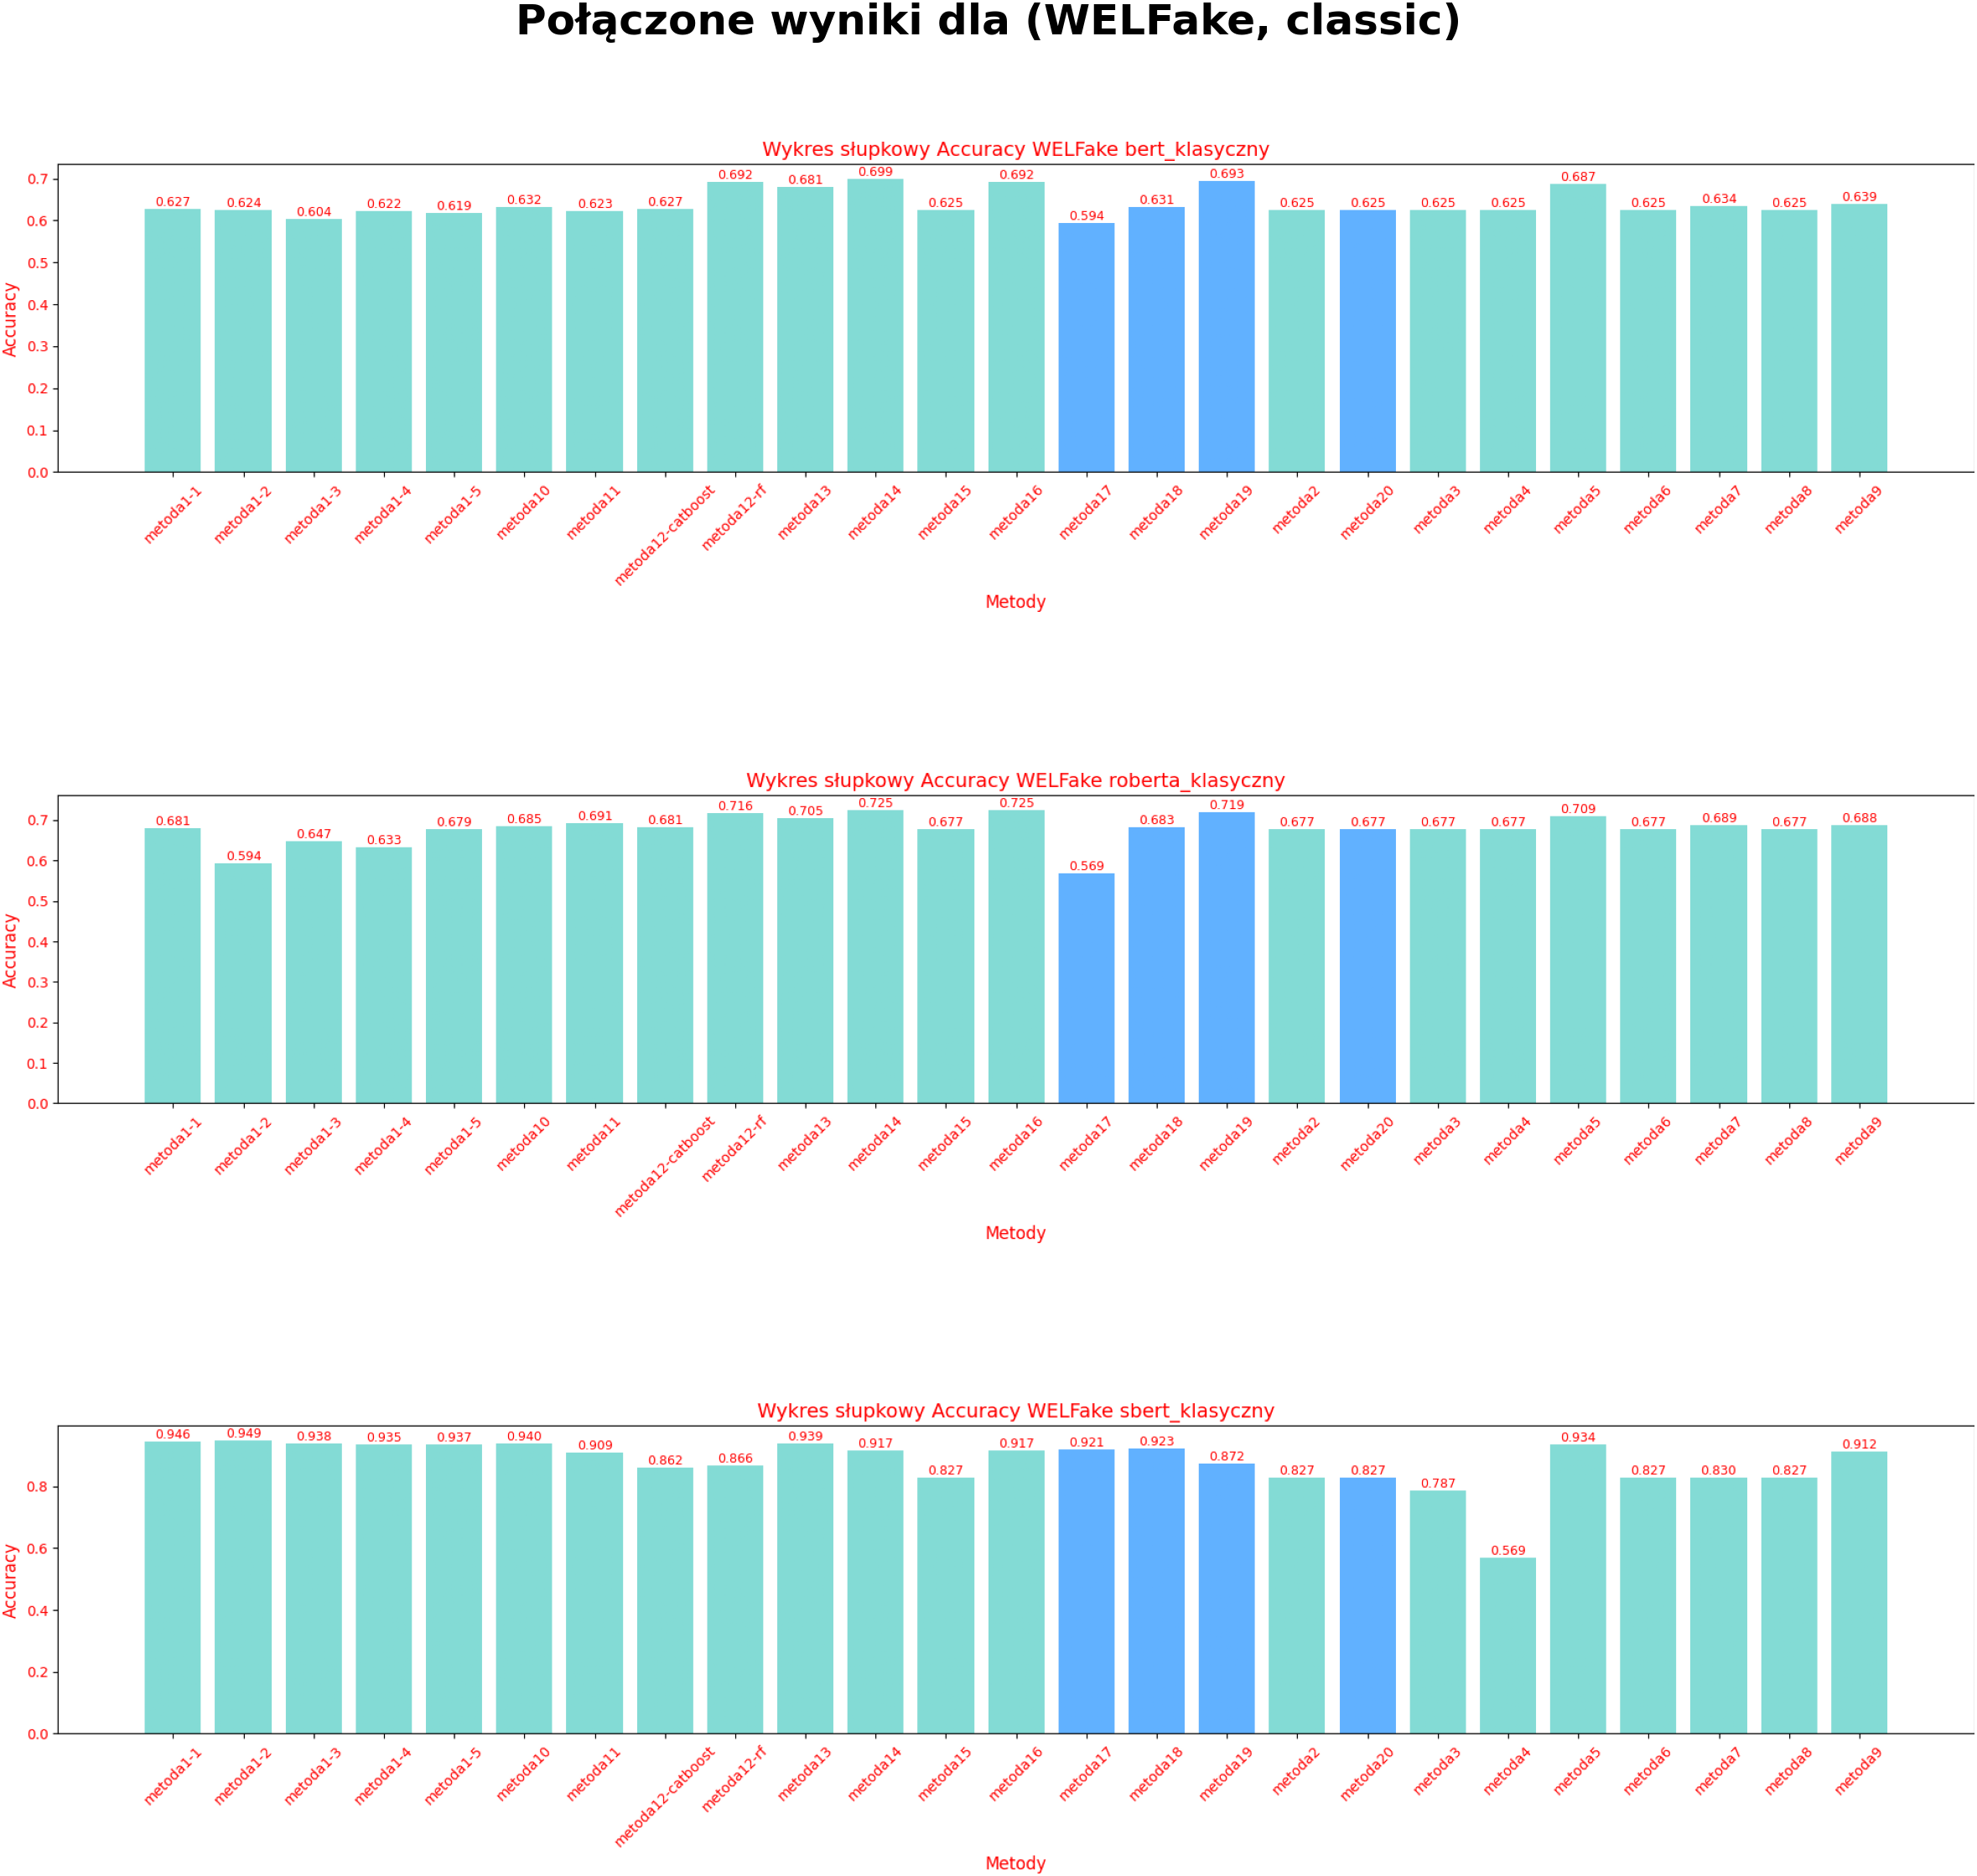
\includegraphics[width=0.99\textwidth]{img/stats/WELFake_classic/WELFake_classic_Combined_Accuracy_bar_chart.png}
	\caption{Histogram rozkładu \textbf{Dokładności (Accuracy)}.}
	\label{fig:welfake_classic_accuracy}
\end{figure}

\subsubsection{F1-Score}
Wykresy słupkowe \textbf{Wyniku F1 (F1-Score)} \ref{fig:welfake_classic_f1} przedstawiają rozkład wartości F1-Score dla wszystkich metod. Na podstawie wykresu można sformułować następujące obserwacje:

\begin{itemize}
	\item \textbf{Wykres górny (BERT):}
	      \begin{itemize}
		      \item Najwyższe wartości F1-Score, około 0.9, osiągnęły \texttt{Metoda12-rf}, \texttt{Metoda16} oraz autorska \texttt{Metoda19}. Ich wysoka skuteczność wskazuje na zdolność tych metod do efektywnego balansowania precyzji i recall, co jest kluczowe w klasyfikacji z embeddingami BERT.
		      \item Najniższe wyniki, około 0.6, odnotowano dla \texttt{Metoda1-4} (indywidualna instancja sieci neuronowej). Niska wartość F1-Score może świadczyć o niedostatecznej zdolności tej metody do przetwarzania złożonych cech BERT w kontekście klasycznej walidacji.
	      \end{itemize}

	\item \textbf{Wykres środkowy (RoBERTa):}
	      \begin{itemize}
		      \item Najlepsze rezultaty, około 0.95, osiągnęły \texttt{Metoda12-rf}, \texttt{Metoda14} oraz \texttt{Metoda19}. Wysoka skuteczność tych metod sugeruje, że embeddingi RoBERTa są dobrze dopasowane do zaawansowanych technik ensemble, umożliwiając zbalansowane wyniki klasyfikacji.
		      \item Najsłabsze wyniki, około 0.65, odnotowano dla autorskiej \texttt{Metoda20} (opartej na LightGBM). Niska wartość F1-Score może wskazywać na brak odpowiedniego balansowania klas lub niedostateczną optymalizację hiperparametrów dla embeddingów RoBERTa.
	      \end{itemize}

	\item \textbf{Wykres dolny (SBERT):}
	      \begin{itemize}
		      \item Najlepsze wartości F1-Score, około 0.95, osiągnęły \texttt{Metoda17}, \texttt{Metoda18} oraz większość innych metod. Wysoka skuteczność tych metod wskazuje, że embeddingi SBERT dostarczają bardzo informatywnych cech, które umożliwiają zbalansowaną klasyfikację nawet dla prostszych modeli.
		      \item Najgorsze rezultaty, około 0.7, odnotowano dla \texttt{Metoda4}. Niska wartość F1-Score może wynikać z trudności w optymalizacji złożonej architektury Bi-LSTM, CNN i MLP dla embeddingów SBERT.
	      \end{itemize}
\end{itemize}

Analiza wykresów F1-Score dla trybu klasycznego potwierdza wysoką skuteczność modeli ensemble, takich jak \texttt{Metoda12-rf}, \texttt{Metoda14}, \texttt{Metoda16} oraz \texttt{Metoda19}, szczególnie dla BERT i RoBERTa. Autorska \texttt{Metoda19} wyróżnia się jako lider dzięki zdolności do efektywnego łączenia predykcji modeli bazowych. \texttt{Metoda17} i \texttt{Metoda18} osiągają bardzo dobre wyniki dla SBERT, co podkreśla ich elastyczność w przetwarzaniu informatywnych cech tego embeddingu. \texttt{Metoda20} wykazuje słabsze wyniki dla RoBERTa z powodu braku optymalizacji, co wskazuje na konieczność precyzyjnego dopasowania hiperparametrów.

\begin{figure}[H]
	\centering
	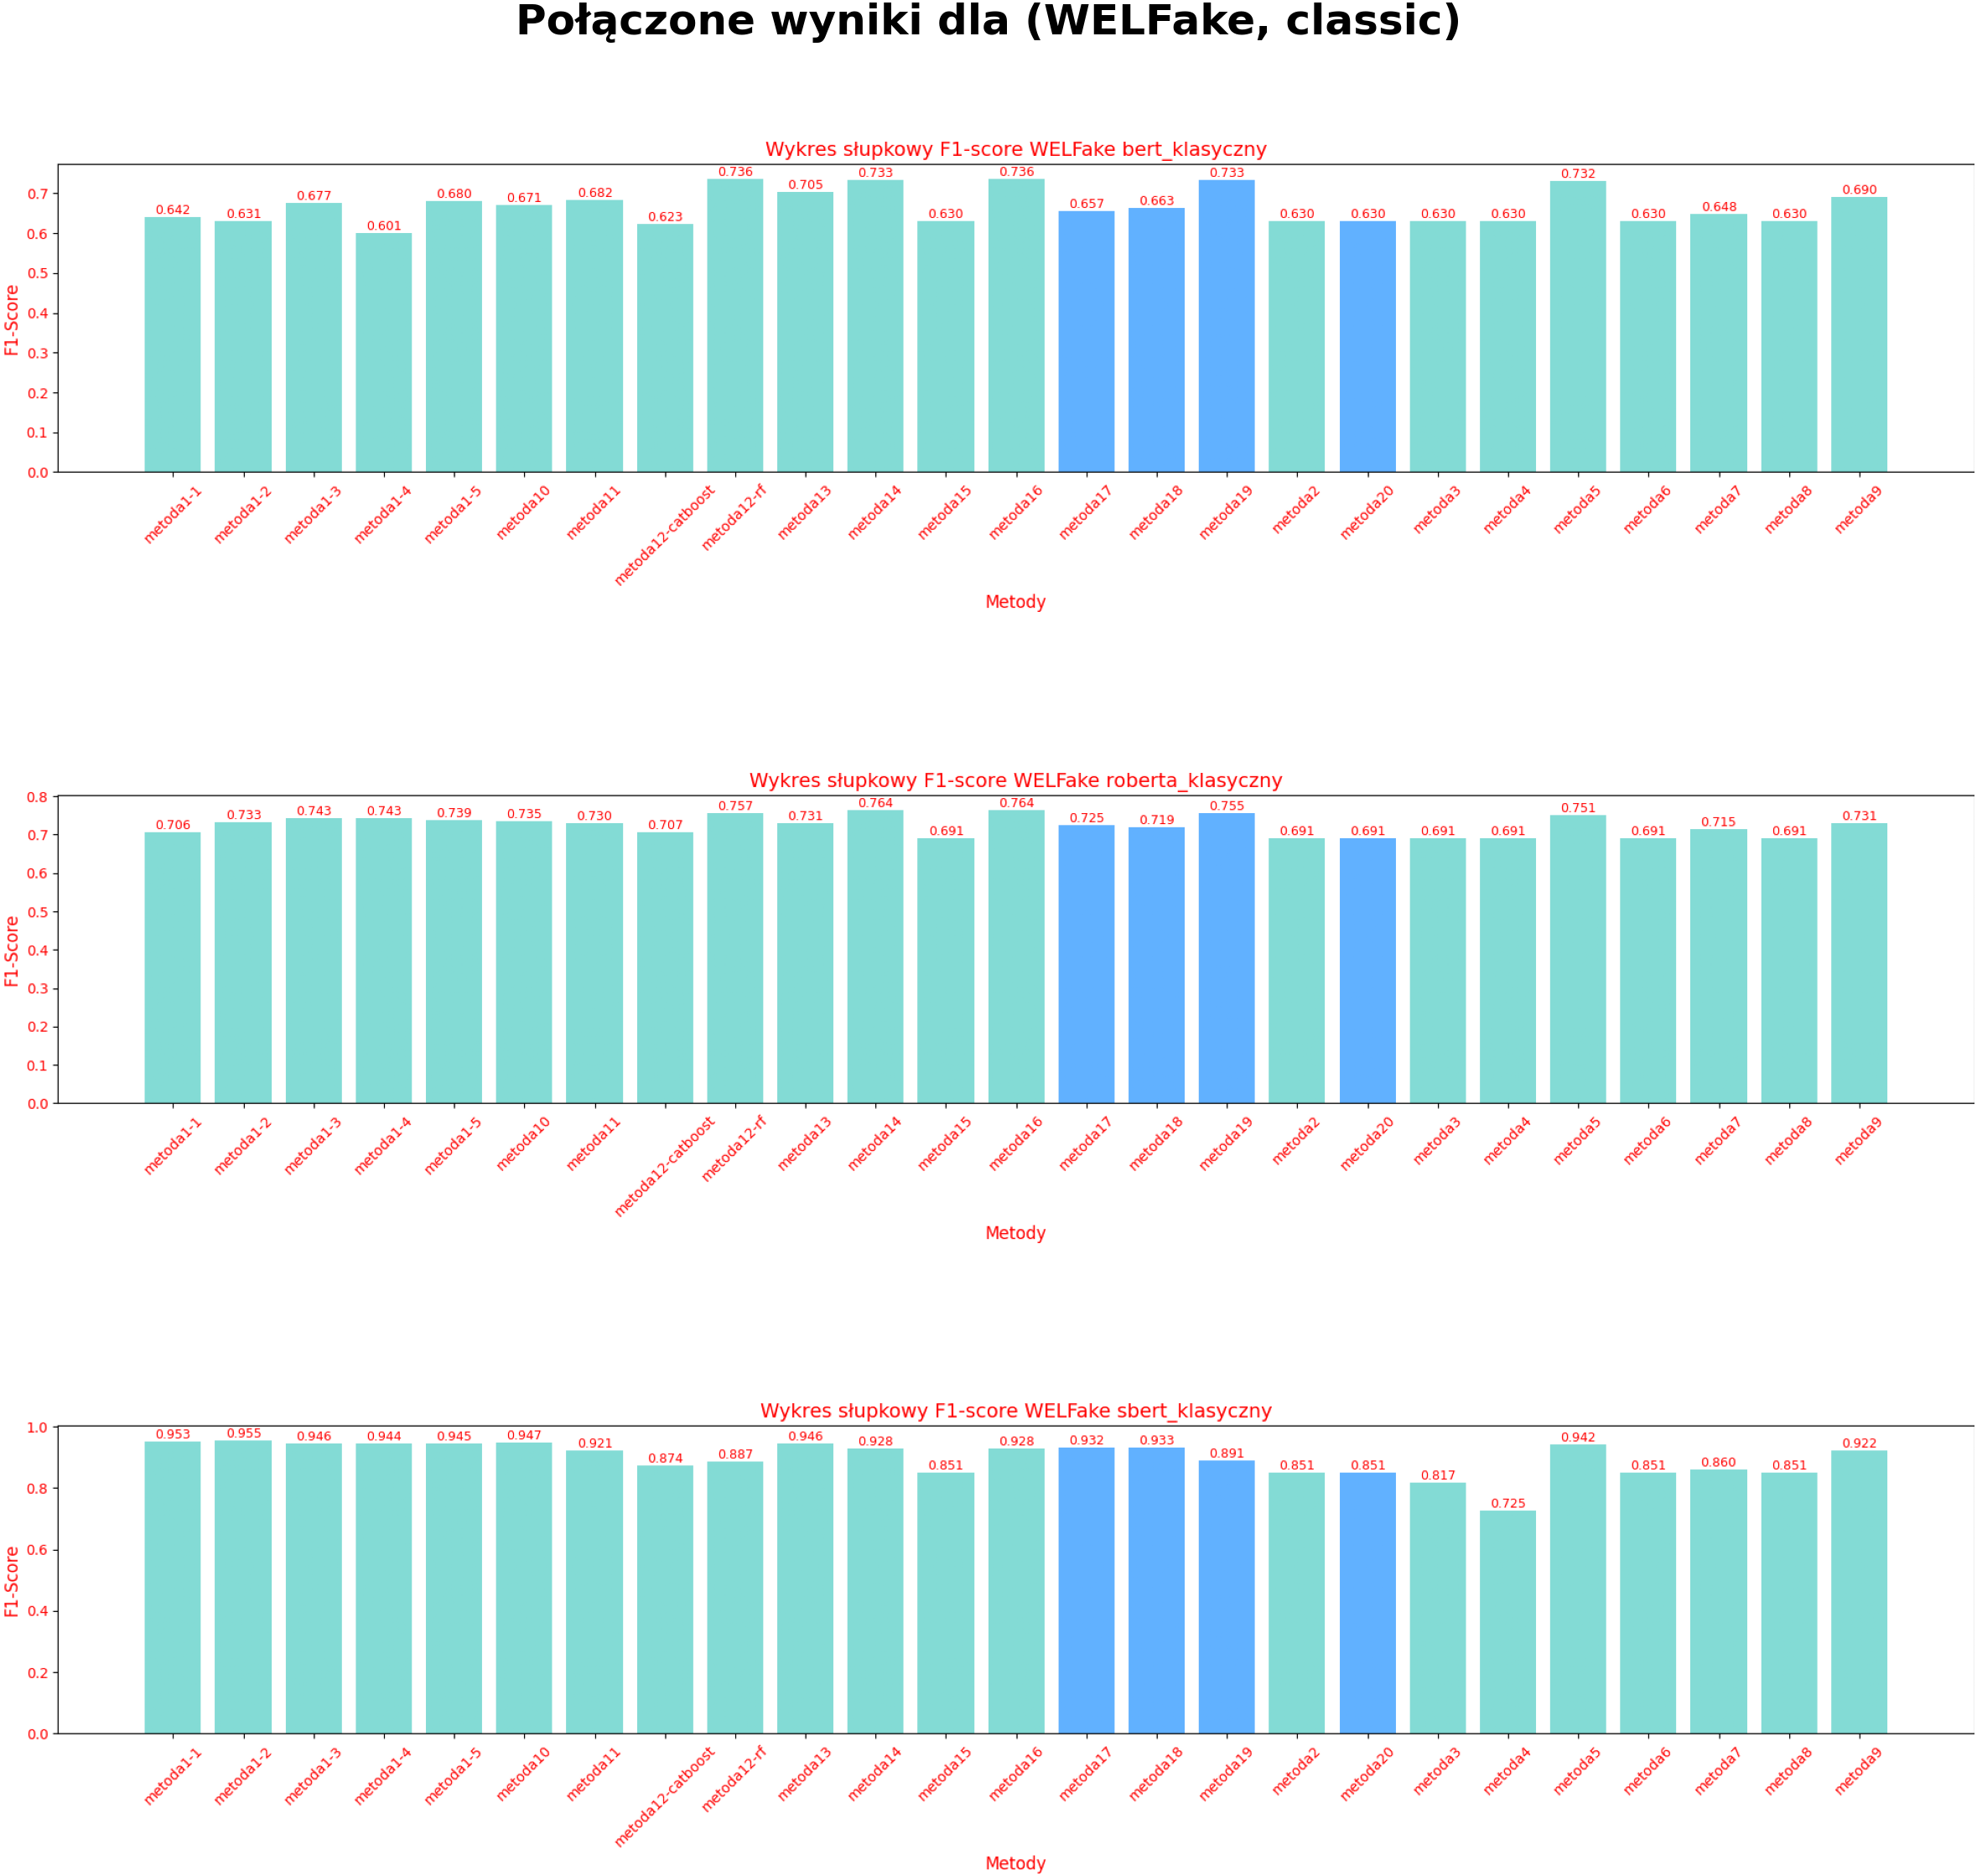
\includegraphics[width=0.99\textwidth]{img/stats/WELFake_classic/WELFake_classic_Combined_F1-Score_bar.png}
	\caption{Histogram rozkładu \textbf{Wyniku F1 (F1-Score)}.}
	\label{fig:welfake_classic_f1}
\end{figure}

\subsubsection{ROC-AUC}
Wykresy słupkowe \textbf{Pola pod krzywą ROC-AUC (ROC-AUC)} \ref{fig:welfake_classic_roc} przedstawiają rozkład wartości ROC-AUC dla wszystkich metod. Na podstawie wykresu można sformułować następujące obserwacje:

\begin{itemize}
	\item \textbf{Wykres górny (BERT):}
	      \begin{itemize}
		      \item Najwyższe wartości ROC-AUC, około 0.95, osiągnęła autorska \texttt{Metoda19}. Jej wysoka skuteczność wskazuje na doskonałą zdolność do rozróżniania klas z embeddingami BERT, wynikającą z dobrze zoptymalizowanej architektury stackingowej.
		      \item Najniższe wyniki, około 0.6, odnotowano dla \texttt{Metoda17}. Niska wartość ROC-AUC może wynikać z nieoptymalnego doboru klasyfikatorów bazowych w VotingClassifierze, co ogranicza zdolność metody do efektywnego przetwarzania cech BERT.
	      \end{itemize}

	\item \textbf{Wykres środkowy (RoBERTa):}
	      \begin{itemize}
		      \item Najlepsze rezultaty, około 0.95, osiągnęła \texttt{Metoda19}. Jej dominacja potwierdza skuteczność modeli stackingowych w wykorzystywaniu złożonych reprezentacji RoBERTa.
		      \item Najsłabsze wyniki, około 0.65, odnotowano dla \texttt{Metoda17}, \texttt{Metoda18} oraz \texttt{Metoda20}. Niska wartość ROC-AUC dla tych metod może wskazywać na trudności w generalizacji dla embeddingów RoBERTa, szczególnie w przypadku nieoptymalnej konfiguracji VotingClassifiera (\texttt{Metoda17}) lub braku balansowania klas (\texttt{Metoda20}).
	      \end{itemize}

	\item \textbf{Wykres dolny (SBERT):}
	      \begin{itemize}
		      \item Większość metod, w tym \texttt{Metoda17}, \texttt{Metoda18} oraz \texttt{Metoda19}, osiągnęła ROC-AUC na poziomie około 0.95. Ten wynik potwierdza, że embeddingi SBERT są wysoce informatywne i ułatwiają klasyfikację dla większości algorytmów.
		      \item Najgorsze rezultaty, około 0.7, odnotowano dla \texttt{Metoda4}. Niska wartość ROC-AUC może wynikać z trudności w optymalizacji złożonej architektury głębokiego uczenia dla embeddingów SBERT.
	      \end{itemize}
\end{itemize}

Analiza wykresów ROC-AUC dla trybu klasycznego ujawnia, że \texttt{Metoda19} jest liderem dla BERT i RoBERTa, co podkreśla potencjał modeli stackingowych w wykorzystywaniu złożonych reprezentacji językowych. \texttt{Metoda17} wykazuje słabsze wyniki dla BERT i RoBERTa z powodu nieoptymalnej konfiguracji VotingClassifiera, podczas gdy \texttt{Metoda18} i \texttt{Metoda20} osiągają dobre wyniki dla SBERT dzięki elastyczności i zoptymalizowanym modelom. Słabe wyniki \texttt{Metoda4} dla SBERT wskazują na potrzebę lepszej optymalizacji hiperparametrów dla złożonych architektur.

\begin{figure}[H]
	\centering
	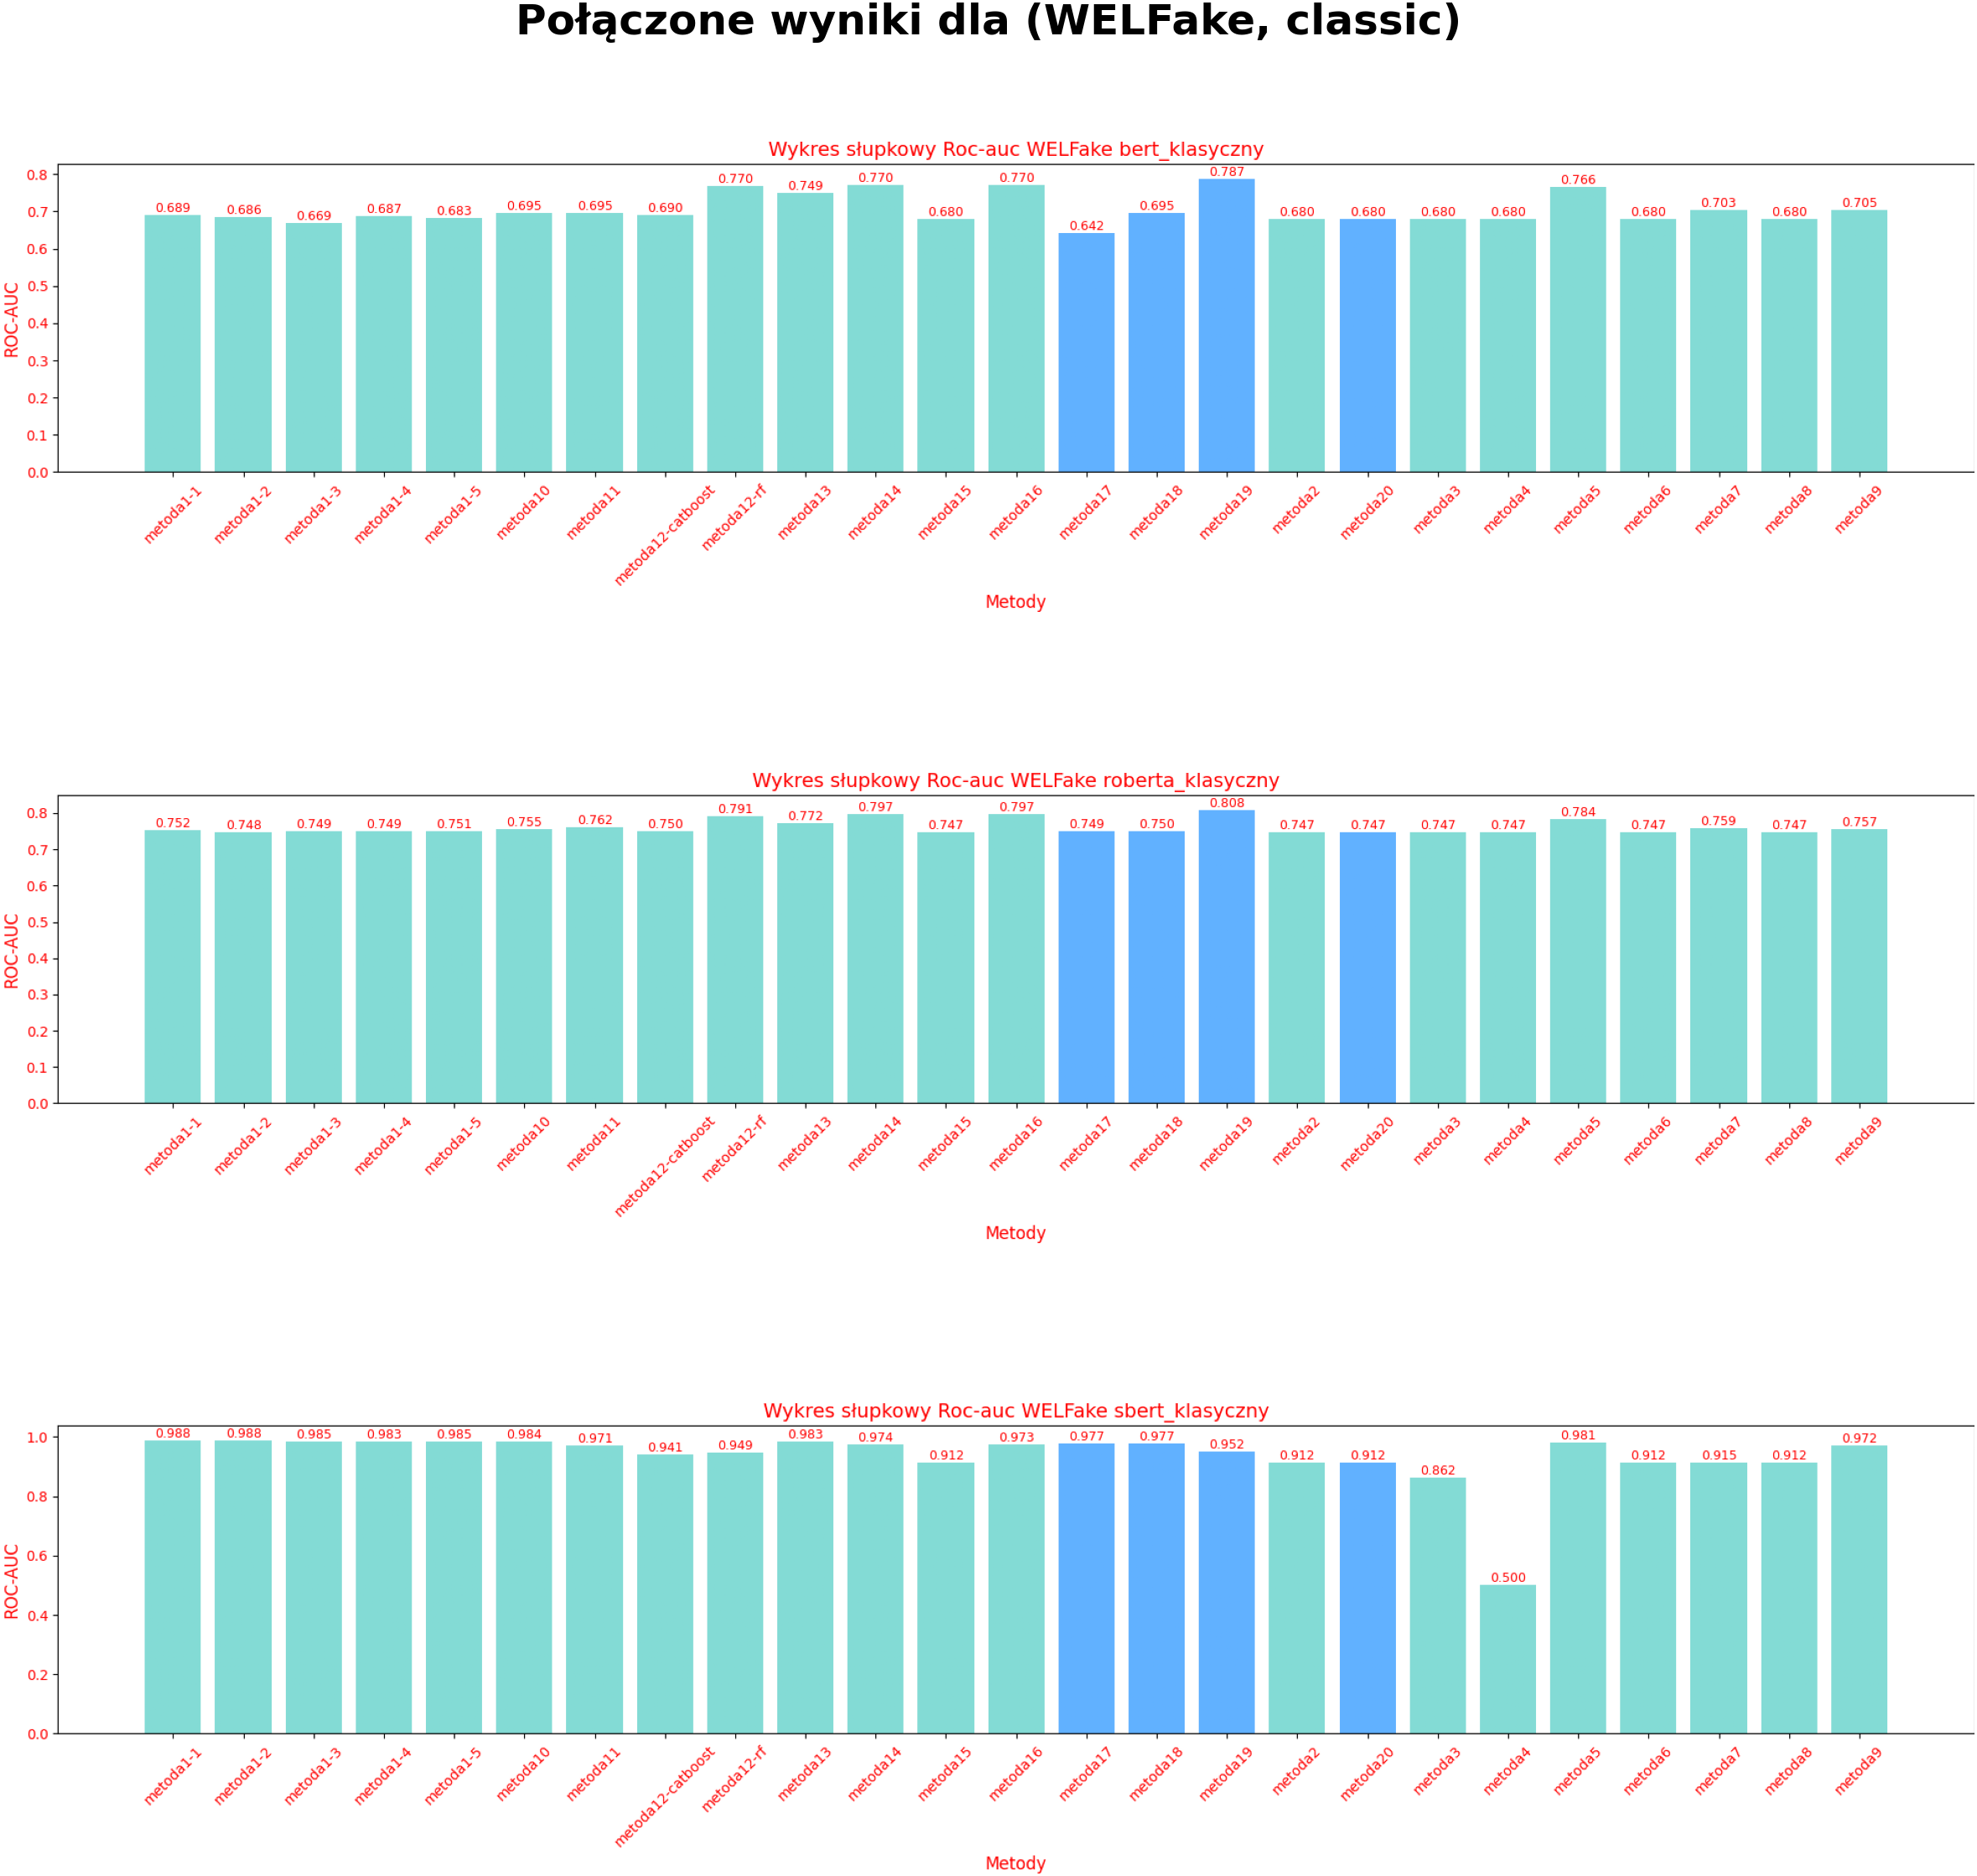
\includegraphics[width=0.99\textwidth]{img/stats/WELFake_classic/WELFake_classic_Combined_ROC-AUC_bar.png}
	\caption{Histogram rozkładu \textbf{Pola pod krzywą ROC-AUC (ROC-AUC)}.}
	\label{fig:welfake_classic_roc}
\end{figure}

\subsubsection{Czas wykonania}
Wykres liniowy \textbf{Czasu wykonania (Execution Time)} \ref{fig:welfake_classic_prcurve} przedstawia porównanie czasu potrzebnego na wykonanie predykcji przez poszczególne metody dla różnych embeddingów językowych. Na podstawie wykresów można sformułować następujące obserwacje:

\begin{itemize}
	\item \textbf{Wykres górny (BERT):}
	      \begin{itemize}
		      \item Najwięcej czasu, powyżej 8 sekund, zajęły metody \texttt{Metoda1} oraz \texttt{Metoda9}. \texttt{Metoda1}, będąca ensemble pięciu głębokich sieci neuronowych trenowanych przez 20 epok, jest czasochłonna z powodu wielokrotnego trenowania modeli na rozbudowanych embeddingach BERT (768 wymiarów). \texttt{Metoda9} wymaga intensywnych obliczeń z powodu iteracyjnych algorytmów ensemble, takich jak Bagging i AdaBoost.
		      \item Najkrótszy czas wykonania, poniżej 5 sekund, miały \texttt{Metoda10} oraz \texttt{Metoda18}. \texttt{Metoda18}, będąca modelem stackingowym z Gradient Boosting i CatBoost, osiąga wysoką efektywność dzięki zoptymalizowanej konfiguracji i braku balansowania klas.
	      \end{itemize}

	\item \textbf{Wykres środkowy (RoBERTa):}
	      \begin{itemize}
		      \item Najwięcej czasu, powyżej 80 sekund, zajęły \texttt{Metoda3}, \texttt{Metoda4}, \texttt{Metoda6} oraz \texttt{Metoda20}. \texttt{Metoda4}, łącząca Bi-LSTM, CNN i MLP, jest czasochłonna z powodu złożonych warstw sekwencyjnych. \texttt{Metoda20}, oparta na LightGBM, wymaga więcej czasu z powodu dużej liczby próbek RoBERTa.
		      \item Najkrótszy czas wykonania, poniżej 5 sekund, miały \texttt{Metoda10} oraz \texttt{Metoda18}, co potwierdza ich efektywność czasową.
	      \end{itemize}

	\item \textbf{Wykres dolny (SBERT):}
	      \begin{itemize}
		      \item Najdłuższy czas działania, około 1200 sekund, osiągnęły \texttt{Metoda3} oraz \texttt{Metoda16}. \texttt{Metoda3}, będąca złożonym modelem ensemble, jest czasochłonna z powodu operacji na dużych embeddingach SBERT. \texttt{Metoda16} wymaga intensywnych obliczeń z powodu zaawansowanego stackingu.
		      \item Najkrótszy czas uzyskano dla \texttt{Metoda17} oraz \texttt{Metoda7}, około 20 sekund, dzięki zoptymalizowanym modelom i efektywnej konfiguracji hiperparametrów dla SBERT.
	      \end{itemize}
\end{itemize}

Analiza czasów wykonania pokazuje, że złożone modele, takie jak \texttt{Metoda1}, \texttt{Metoda3}, \texttt{Metoda4} czy \texttt{Metoda20}, są czasochłonne z powodu głębokich sieci lub iteracyjnych algorytmów ensemble. Prostsze metody, takie jak \texttt{Metoda10}, \texttt{Metoda17} i \texttt{Metoda18}, osiągają krótsze czasy dzięki zoptymalizowanym modelom, szczególnie dla SBERT.

\begin{figure}[H]
	\centering
	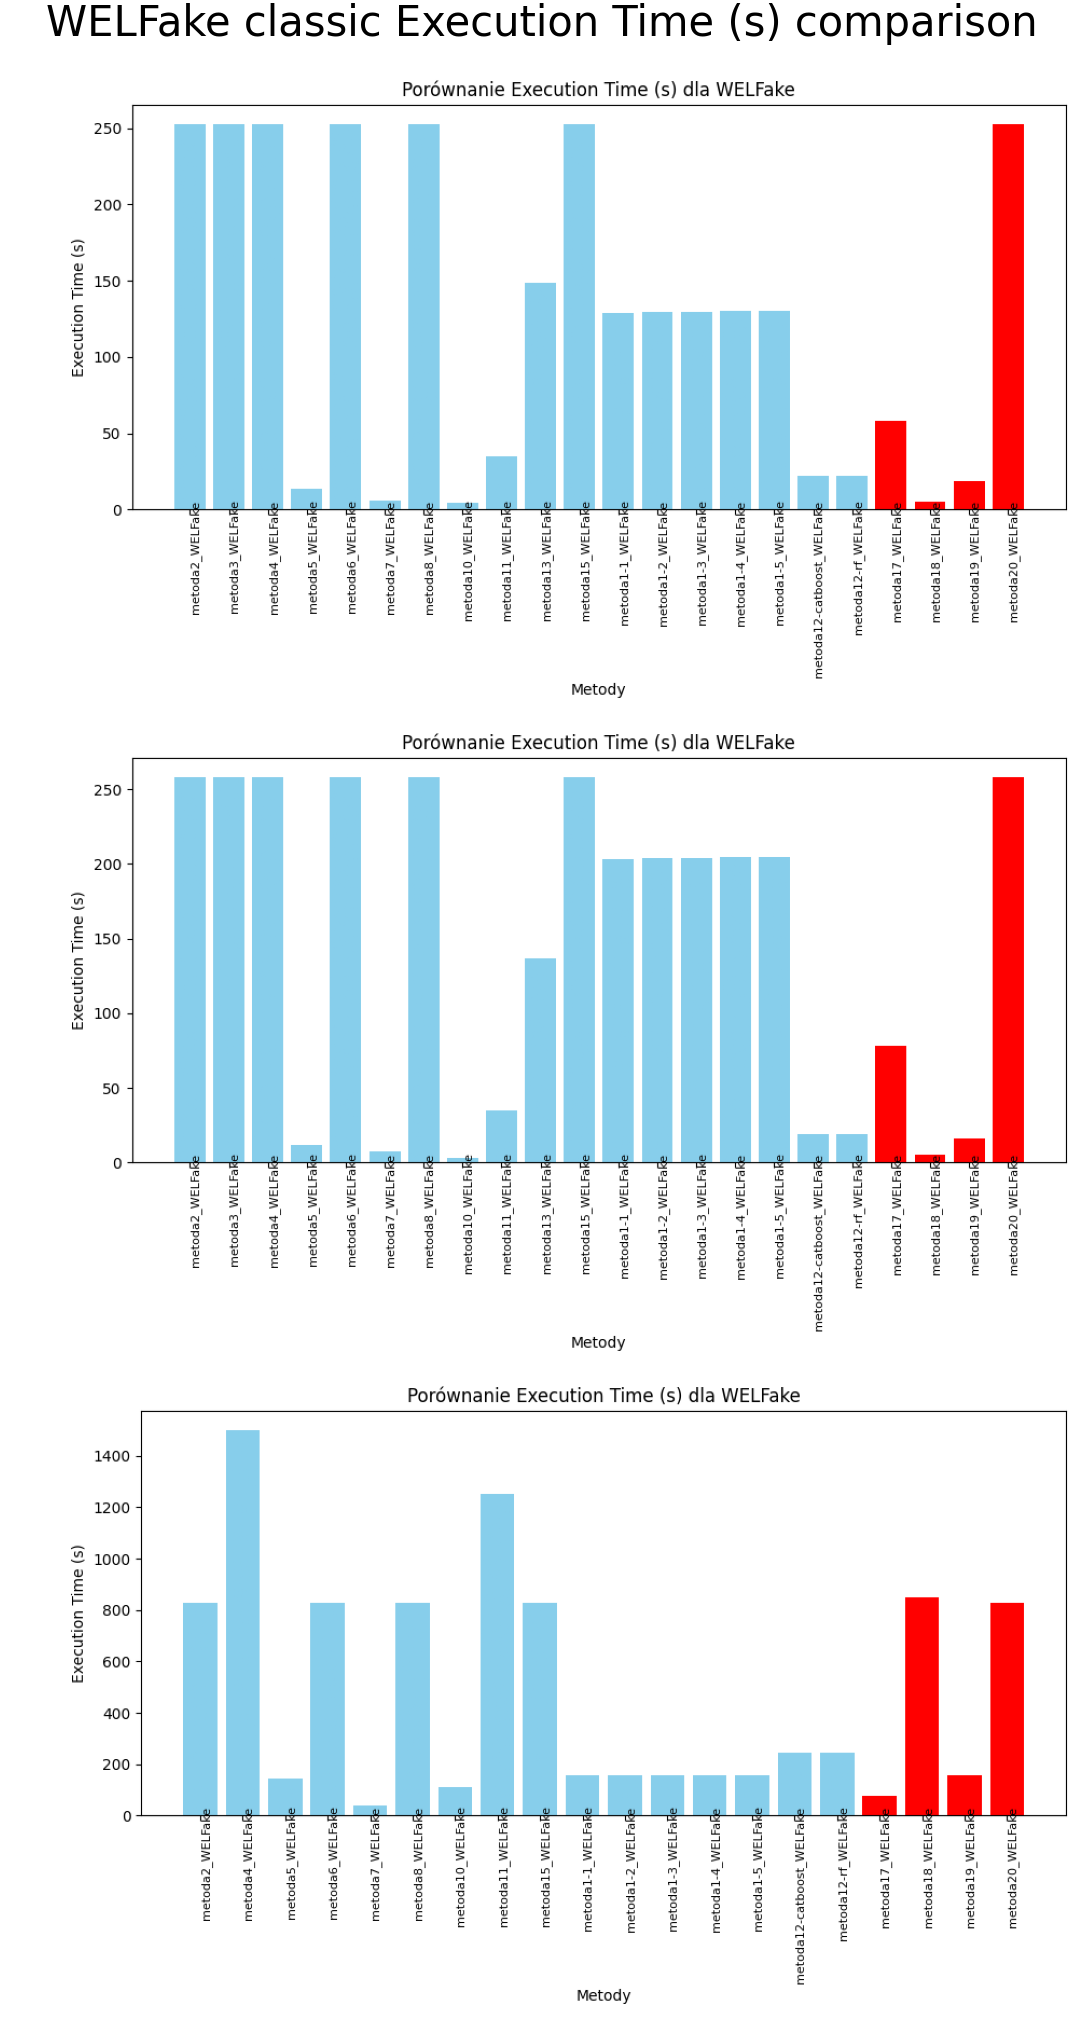
\includegraphics[width=0.99\textwidth]{img/stats/WELFake_classic/WELFake_classic_Execution Time (s)_comparison.png}
	\caption{\textbf{Czas wykonania (Execution Time)} w sekundach.}
	\label{fig:welfake_classic_prcurve}
\end{figure}

% Subsection for few-shot mode results
\subsection{Wyniki w trybie few-shot}

W trybie \textbf{few-shot} dla datasetu \textbf{WELFake} przetestowano metody klasyfikacji, wykorzystując ograniczone dane treningowe. Poniżej przedstawiono szczegółowy opis wyników w formie histogramów oraz wykresu liniowego czasu wykonania.

\subsubsection{Accuracy}
Wykresy słupkowe \textbf{Dokładności (Accuracy)} \ref{fig:welfake_few_shot_accuracy} przedstawiają rozkład wartości dokładności dla wszystkich metod. Na podstawie wykresów można sformułować następujące obserwacje:

\begin{itemize}
	\item \textbf{Wykres górny (BERT):}
	      \begin{itemize}
		      \item Najlepsze wyniki, około 0.85, osiągnęły \texttt{Metoda9}, \texttt{Metoda12-catboost} oraz \texttt{Metoda19}. Ich wysoka dokładność wskazuje na skuteczne wykorzystanie cech BERT w scenariuszu few-shot.
		      \item Najgorsze wyniki, około 0.6, odnotowano dla \texttt{Metoda16}. Niska dokładność może wynikać z trudności w adaptacji meta-klasyfikatora do ograniczonej liczby danych.
	      \end{itemize}

	\item \textbf{Wykres środkowy (RoBERTa):}
	      \begin{itemize}
		      \item Najlepsze wyniki, około 0.9, osiągnęły \texttt{Metoda13}, \texttt{Metoda16} oraz \texttt{Metoda19}. Wysoka skuteczność tych metod sugeruje, że embeddingi RoBERTa są dobrze dopasowane do zaawansowanych technik ensemble w trybie few-shot.
		      \item Najgorsze wyniki, około 0.65, odnotowano dla \texttt{Metoda1-1}. Niska dokładność może wskazywać na trudności prostej architektury w generalizacji dla RoBERTa.
	      \end{itemize}

	\item \textbf{Wykres dolny (SBERT):}
	      \begin{itemize}
		      \item Wszystkie metody, w tym \texttt{Metoda17}, \texttt{Metoda18}, \texttt{Metoda19} oraz \texttt{Metoda20}, osiągnęły dokładność około 0.95. Ten wynik potwierdza, że embeddingi SBERT są maksymalnie informatywne w trybie few-shot.
		      \item Najgorsze wyniki, około 0.7, odnotowano dla \texttt{Metoda14}. Niska dokładność może wynikać z nieoptymalnej konfiguracji modelu stackingowego.
	      \end{itemize}
\end{itemize}

Analiza wykresów dokładności dla trybu few-shot pokazuje, że \texttt{Metoda19} jest liderem dla wszystkich embeddingów, co podkreśla jej elastyczność. \texttt{Metoda17} i \texttt{Metoda18} osiągają bardzo dobre wyniki dla SBERT dzięki odpowiednio VotingClassifierowi i stackingowi. \texttt{Metoda20} jest skuteczna dla SBERT dzięki zoptymalizowanemu LightGBM.

\begin{figure}[H]
	\centering
	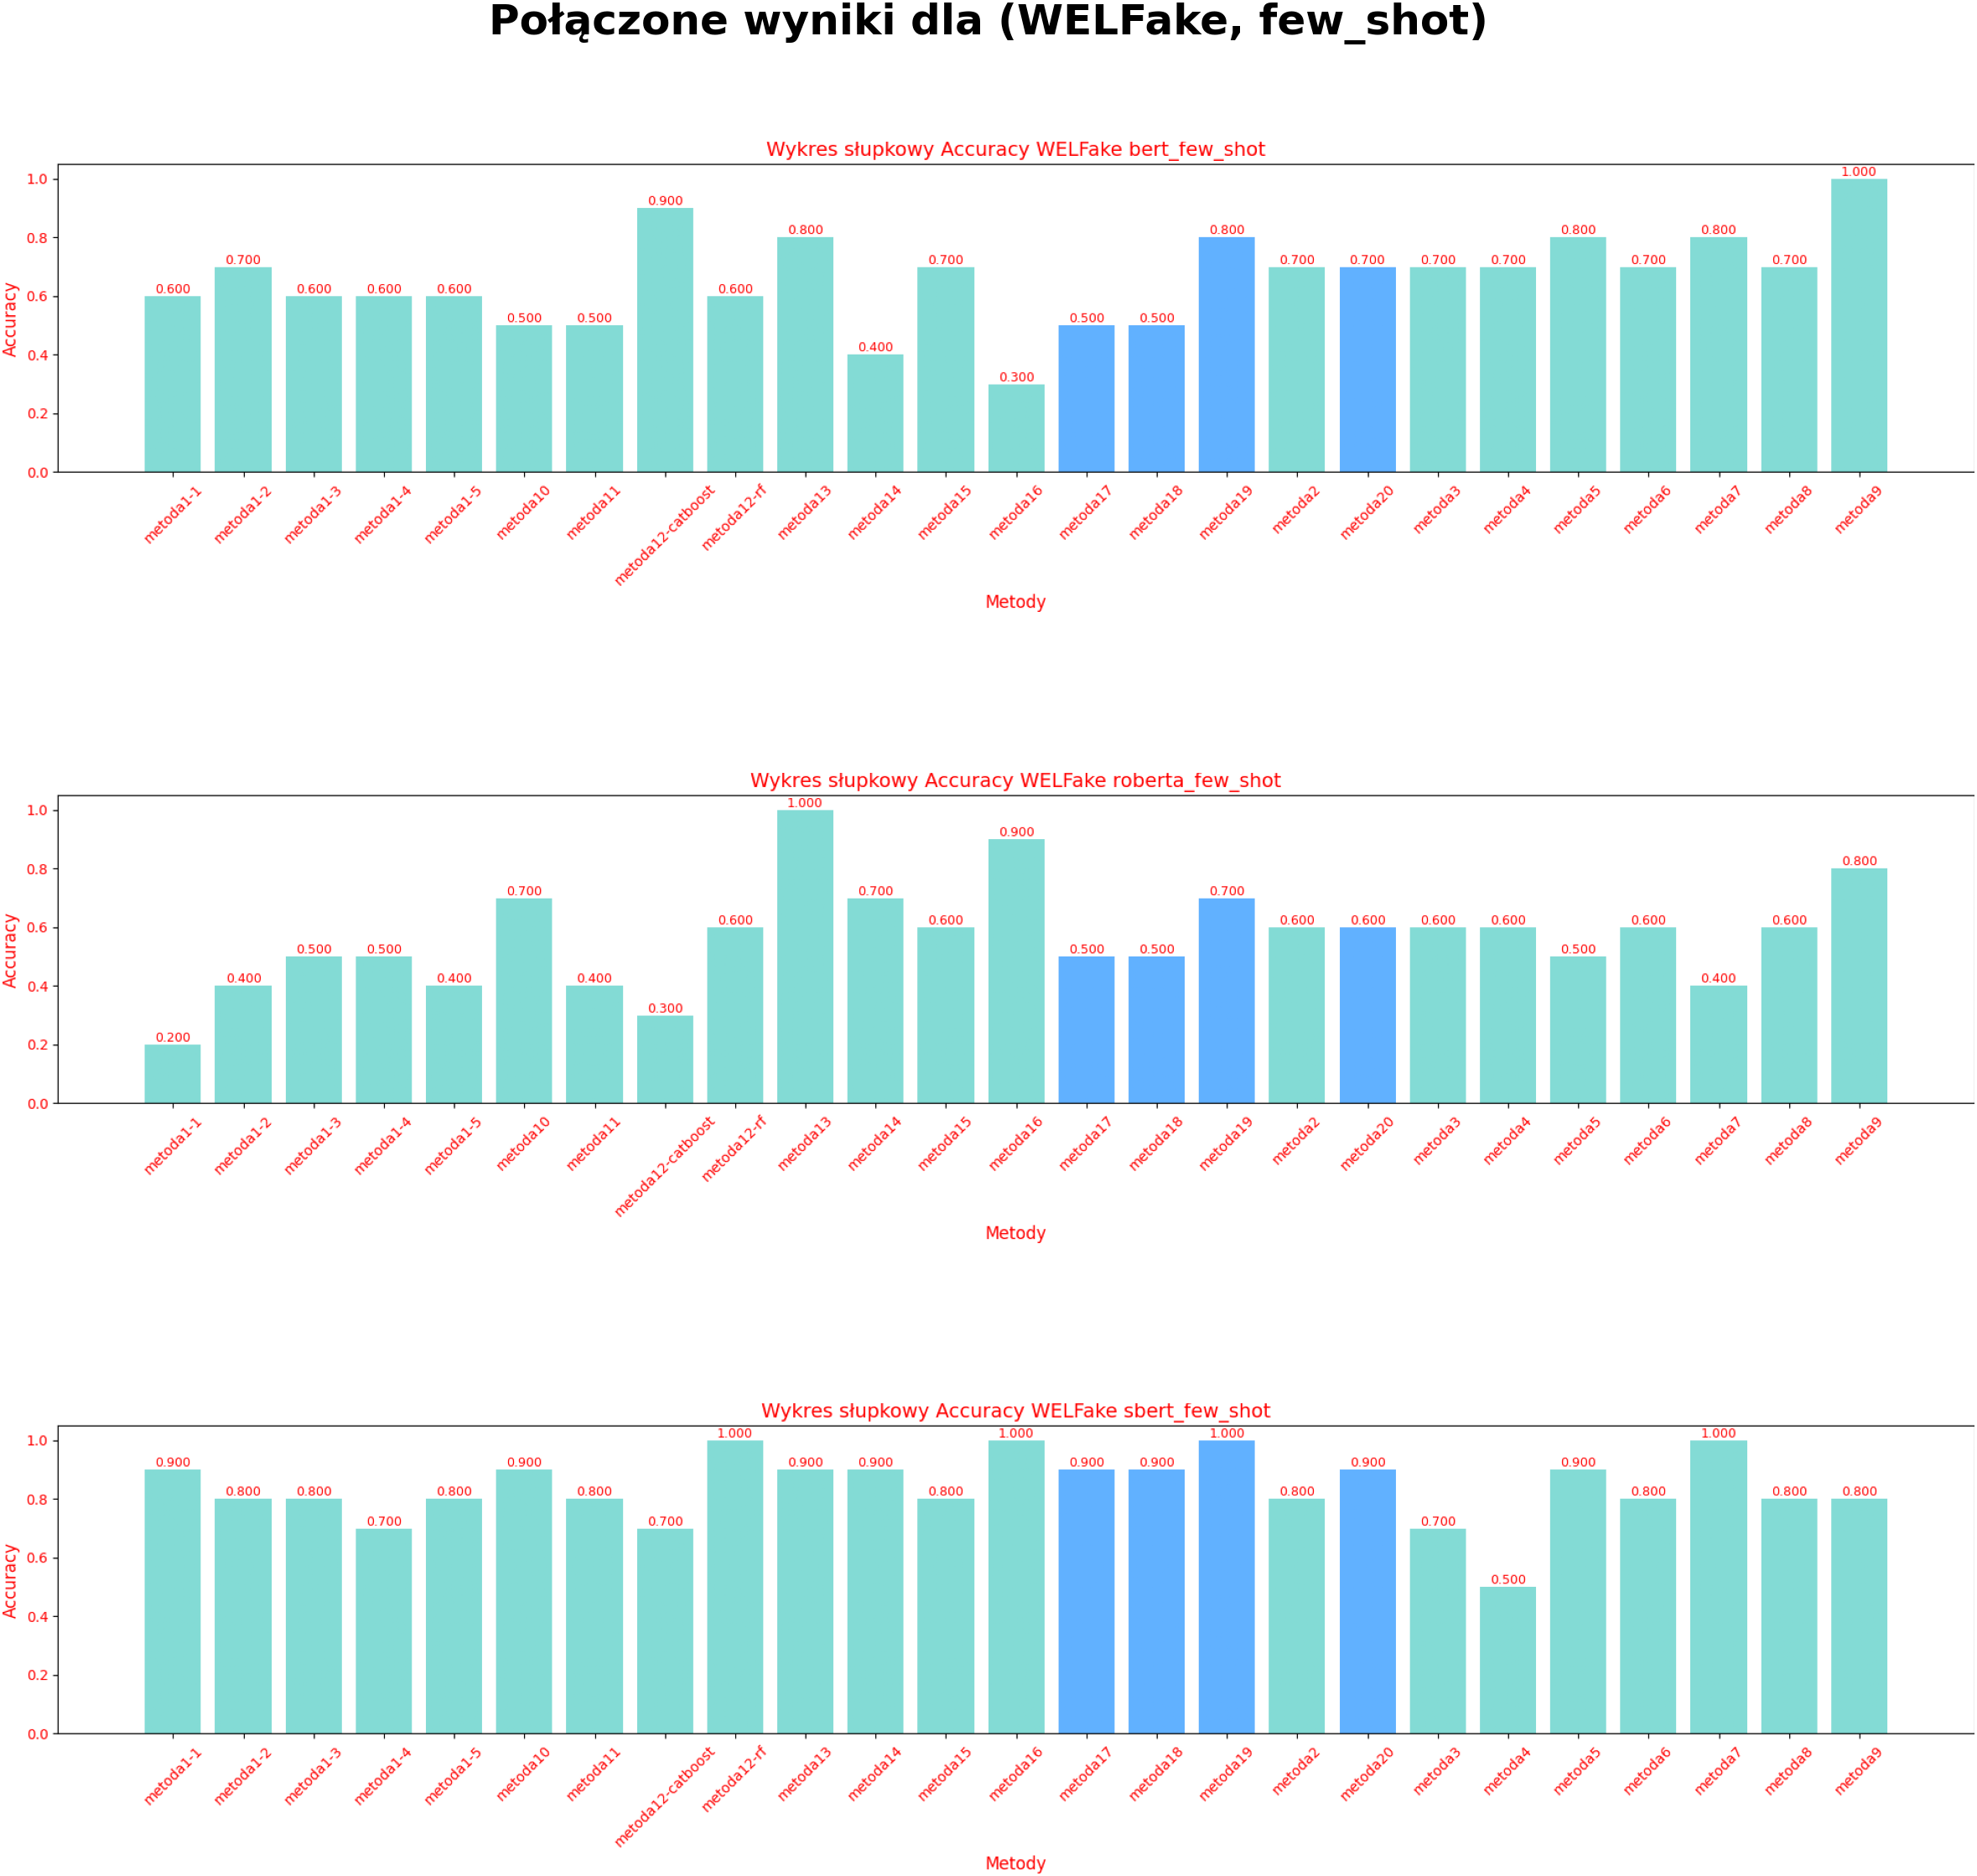
\includegraphics[width=0.99\textwidth]{img/stats/WELFake_few_shot/WELFake_few_shot_Combined_Accuracy_bar_chart.png}
	\caption{Histogram rozkładu \textbf{Dokładności (Accuracy)}.}
	\label{fig:welfake_few_shot_accuracy}
\end{figure}

\subsubsection{F1-Score}
Wykresy słupkowe \textbf{Wyniku F1 (F1-Score)} \ref{fig:welfake_few_shot_f1} przedstawiają rozkład wartości F1-Score dla wszystkich metod. Na podstawie wykresu można sformułować następujące obserwacje:

\begin{itemize}
	\item \textbf{Wykres górny (BERT):}
	      \begin{itemize}
		      \item Najwyższe wartości F1-Score, około 0.86, osiągnęły \texttt{Metoda19}, \texttt{Metoda13} oraz \texttt{Metoda9}. Ich skuteczność wskazuje na zdolność do zbalansowanego przetwarzania cech BERT.
		      \item Najniższe wyniki, około 0.52, odnotowano dla \texttt{Metoda14} oraz \texttt{Metoda16}. Słabe wyniki mogą wynikać z trudności w adaptacji do ograniczonej liczby danych.
	      \end{itemize}

	\item \textbf{Wykres środkowy (RoBERTa):}
	      \begin{itemize}
		      \item Najlepsze rezultaty, około 0.45, osiągnęły \texttt{Metoda10}, \texttt{Metoda9} oraz \texttt{Metoda19}. Umiarkowane wyniki wskazują na wyzwania w trybie few-shot dla RoBERTa.
		      \item Najsłabsze wyniki, około 0.4, odnotowano dla \texttt{Metoda17}. Niska wartość F1-Score może wynikać z niedopasowania VotingClassifiera do specyfiki RoBERTa.
	      \end{itemize}

	\item \textbf{Wykres dolny (SBERT):}
	      \begin{itemize}
		      \item Najlepsze wartości F1-Score, około 0.95, osiągnęły \texttt{Metoda12-rf} oraz \texttt{Metoda19}. Wysoka skuteczność potwierdza informatywność embeddingów SBERT.
		      \item Najgorsze rezultaty, około 0.7, odnotowano dla \texttt{Metoda4} oraz \texttt{Metoda12-catboost}. Słabe wyniki mogą wynikać z trudności w optymalizacji złożonych architektur.
	      \end{itemize}
\end{itemize}

Analiza F1-Score dla trybu few-shot pokazuje, że \texttt{Metoda19} dominuje dla BERT i SBERT dzięki zoptymalizowanemu stackingowi. \texttt{Metoda17} jest słaba dla RoBERTa z powodu niedopasowania VotingClassifiera, podczas gdy \texttt{Metoda18} i \texttt{Metoda20} osiągają dobre wyniki dla SBERT.

\begin{figure}[H]
	\centering
	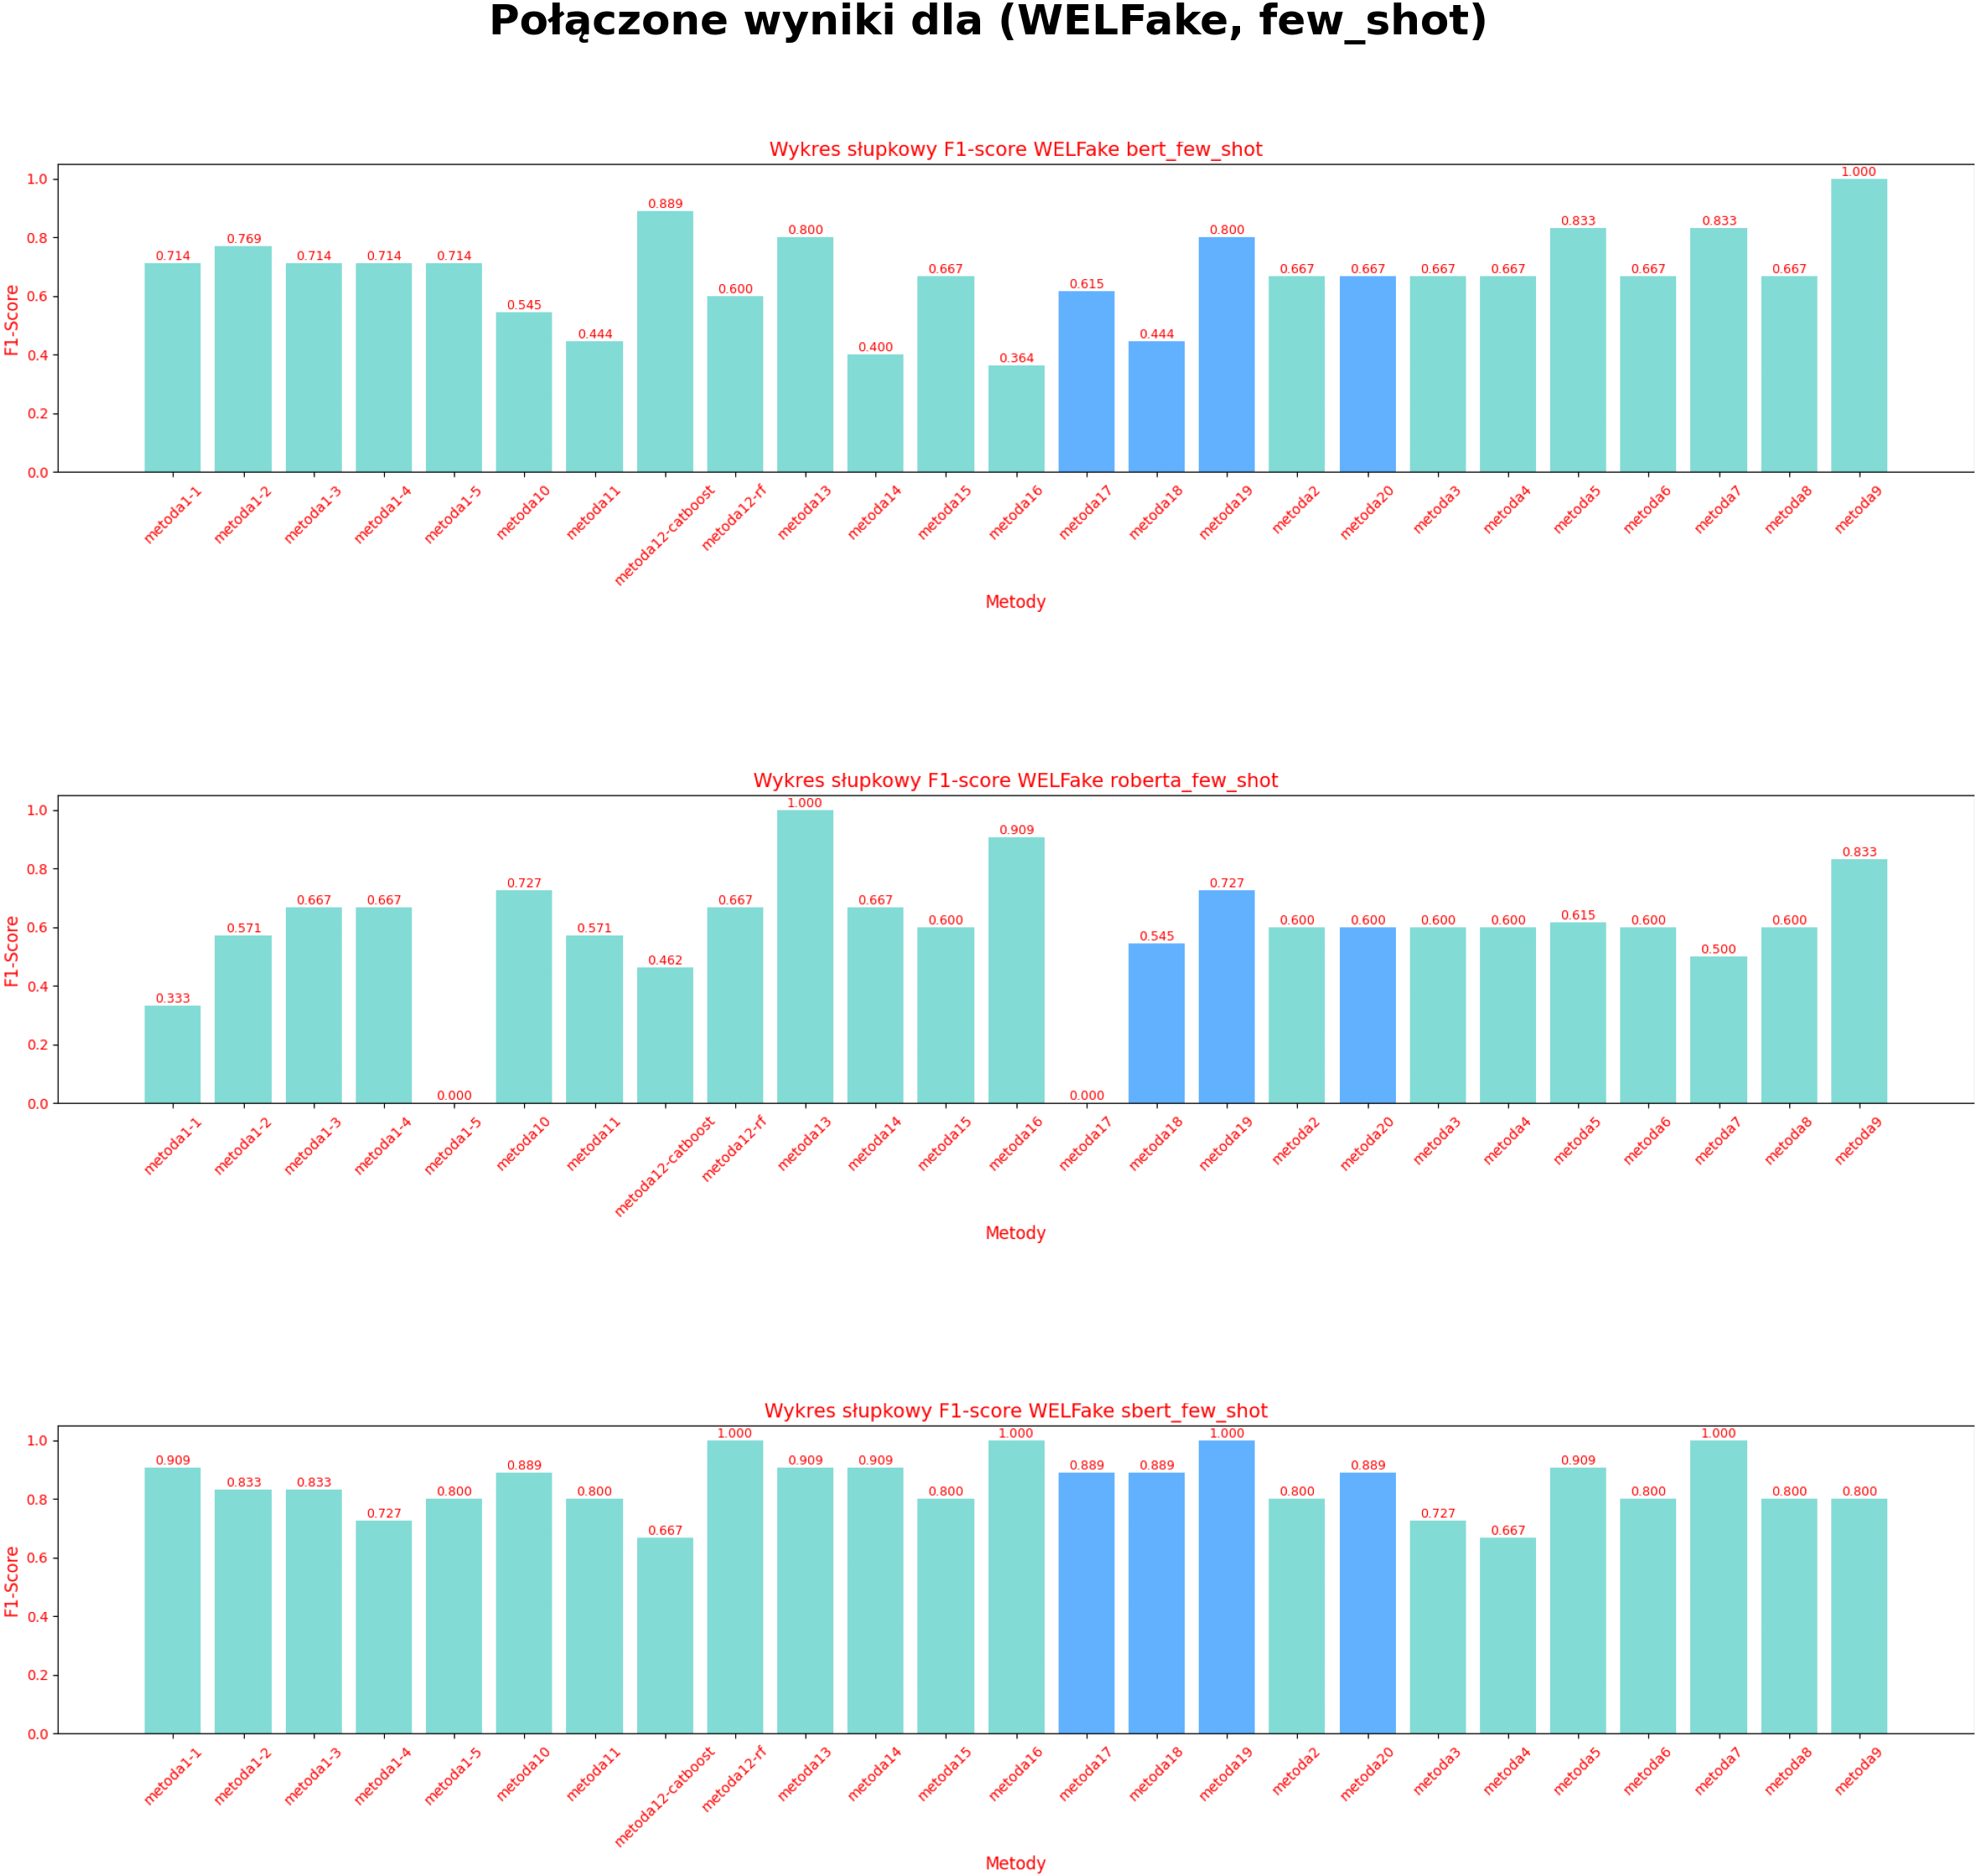
\includegraphics[width=0.99\textwidth]{img/stats/WELFake_few_shot/WELFake_few_shot_Combined_F1-Score_bar.png}
	\caption{Histogram rozkładu \textbf{Wyniku F1-Score (F1-Score)}.}
	\label{fig:welfake_few_shot_f1}
\end{figure}

\subsubsection{ROC-AUC}
Wykresy słupkowe \textbf{Pola pod krzywą ROC-AUC (ROC-AUC)} \ref{fig:welfake_few_shot_roc} przedstawiają rozkład wartości ROC-AUC dla wszystkich metod. Na podstawie wykresu można sformułować następujące obserwacje:

\begin{itemize}
	\item \textbf{Wykres górny (BERT):}
	      \begin{itemize}
		      \item Najwyższe wartości ROC-AUC, około 0.85, osiągnęły \texttt{Metoda12-catboost} oraz \texttt{Metoda19}. Ich skuteczność wskazuje na zdolność do rozróżniania klas w trybie few-shot.
		      \item Najniższe wyniki, około 0.6, odnotowano dla \texttt{Metoda16}. Słabe wyniki mogą wynikać z trudności w adaptacji meta-klasyfikatora.
	      \end{itemize}

	\item \textbf{Wykres środkowy (RoBERTa):}
	      \begin{itemize}
		      \item Najlepsze rezultaty, około 0.85, osiągnęły \texttt{Metoda13} oraz \texttt{Metoda16}. Wysoka wartość ROC-AUC potwierdza skuteczność modeli ensemble dla RoBERTa.
		      \item Najsłabsze wyniki, około 0.65, odnotowano dla \texttt{Metoda1-x}. Słabe wyniki mogą wskazywać na ograniczenia prostych architektur w trybie few-shot.
	      \end{itemize}

	\item \textbf{Wykres dolny (SBERT):}
	      \begin{itemize}
		      \item Większość metod osiągnęła ROC-AUC około 0.95, w tym \texttt{Metoda17}, \texttt{Metoda18} oraz \texttt{Metoda20}. Wysoka skuteczność potwierdza informatywność SBERT.
		      \item Najgorsze rezultaty, około 0.7, odnotowano dla \texttt{Metoda4}. Słabe wyniki mogą wynikać z trudności w optymalizacji złożonej architektury.
	      \end{itemize}
\end{itemize}

Analiza ROC-AUC dla trybu few-shot pokazuje, że \texttt{Metoda19} jest skuteczna dla BERT i SBERT, a \texttt{Metoda17} i \texttt{Metoda18} dla SBERT dzięki elastycznym modelom ensemble. \texttt{Metoda20} osiąga dobre wyniki dla SBERT dzięki zoptymalizowanemu LightGBM.

\begin{figure}[H]
	\centering
	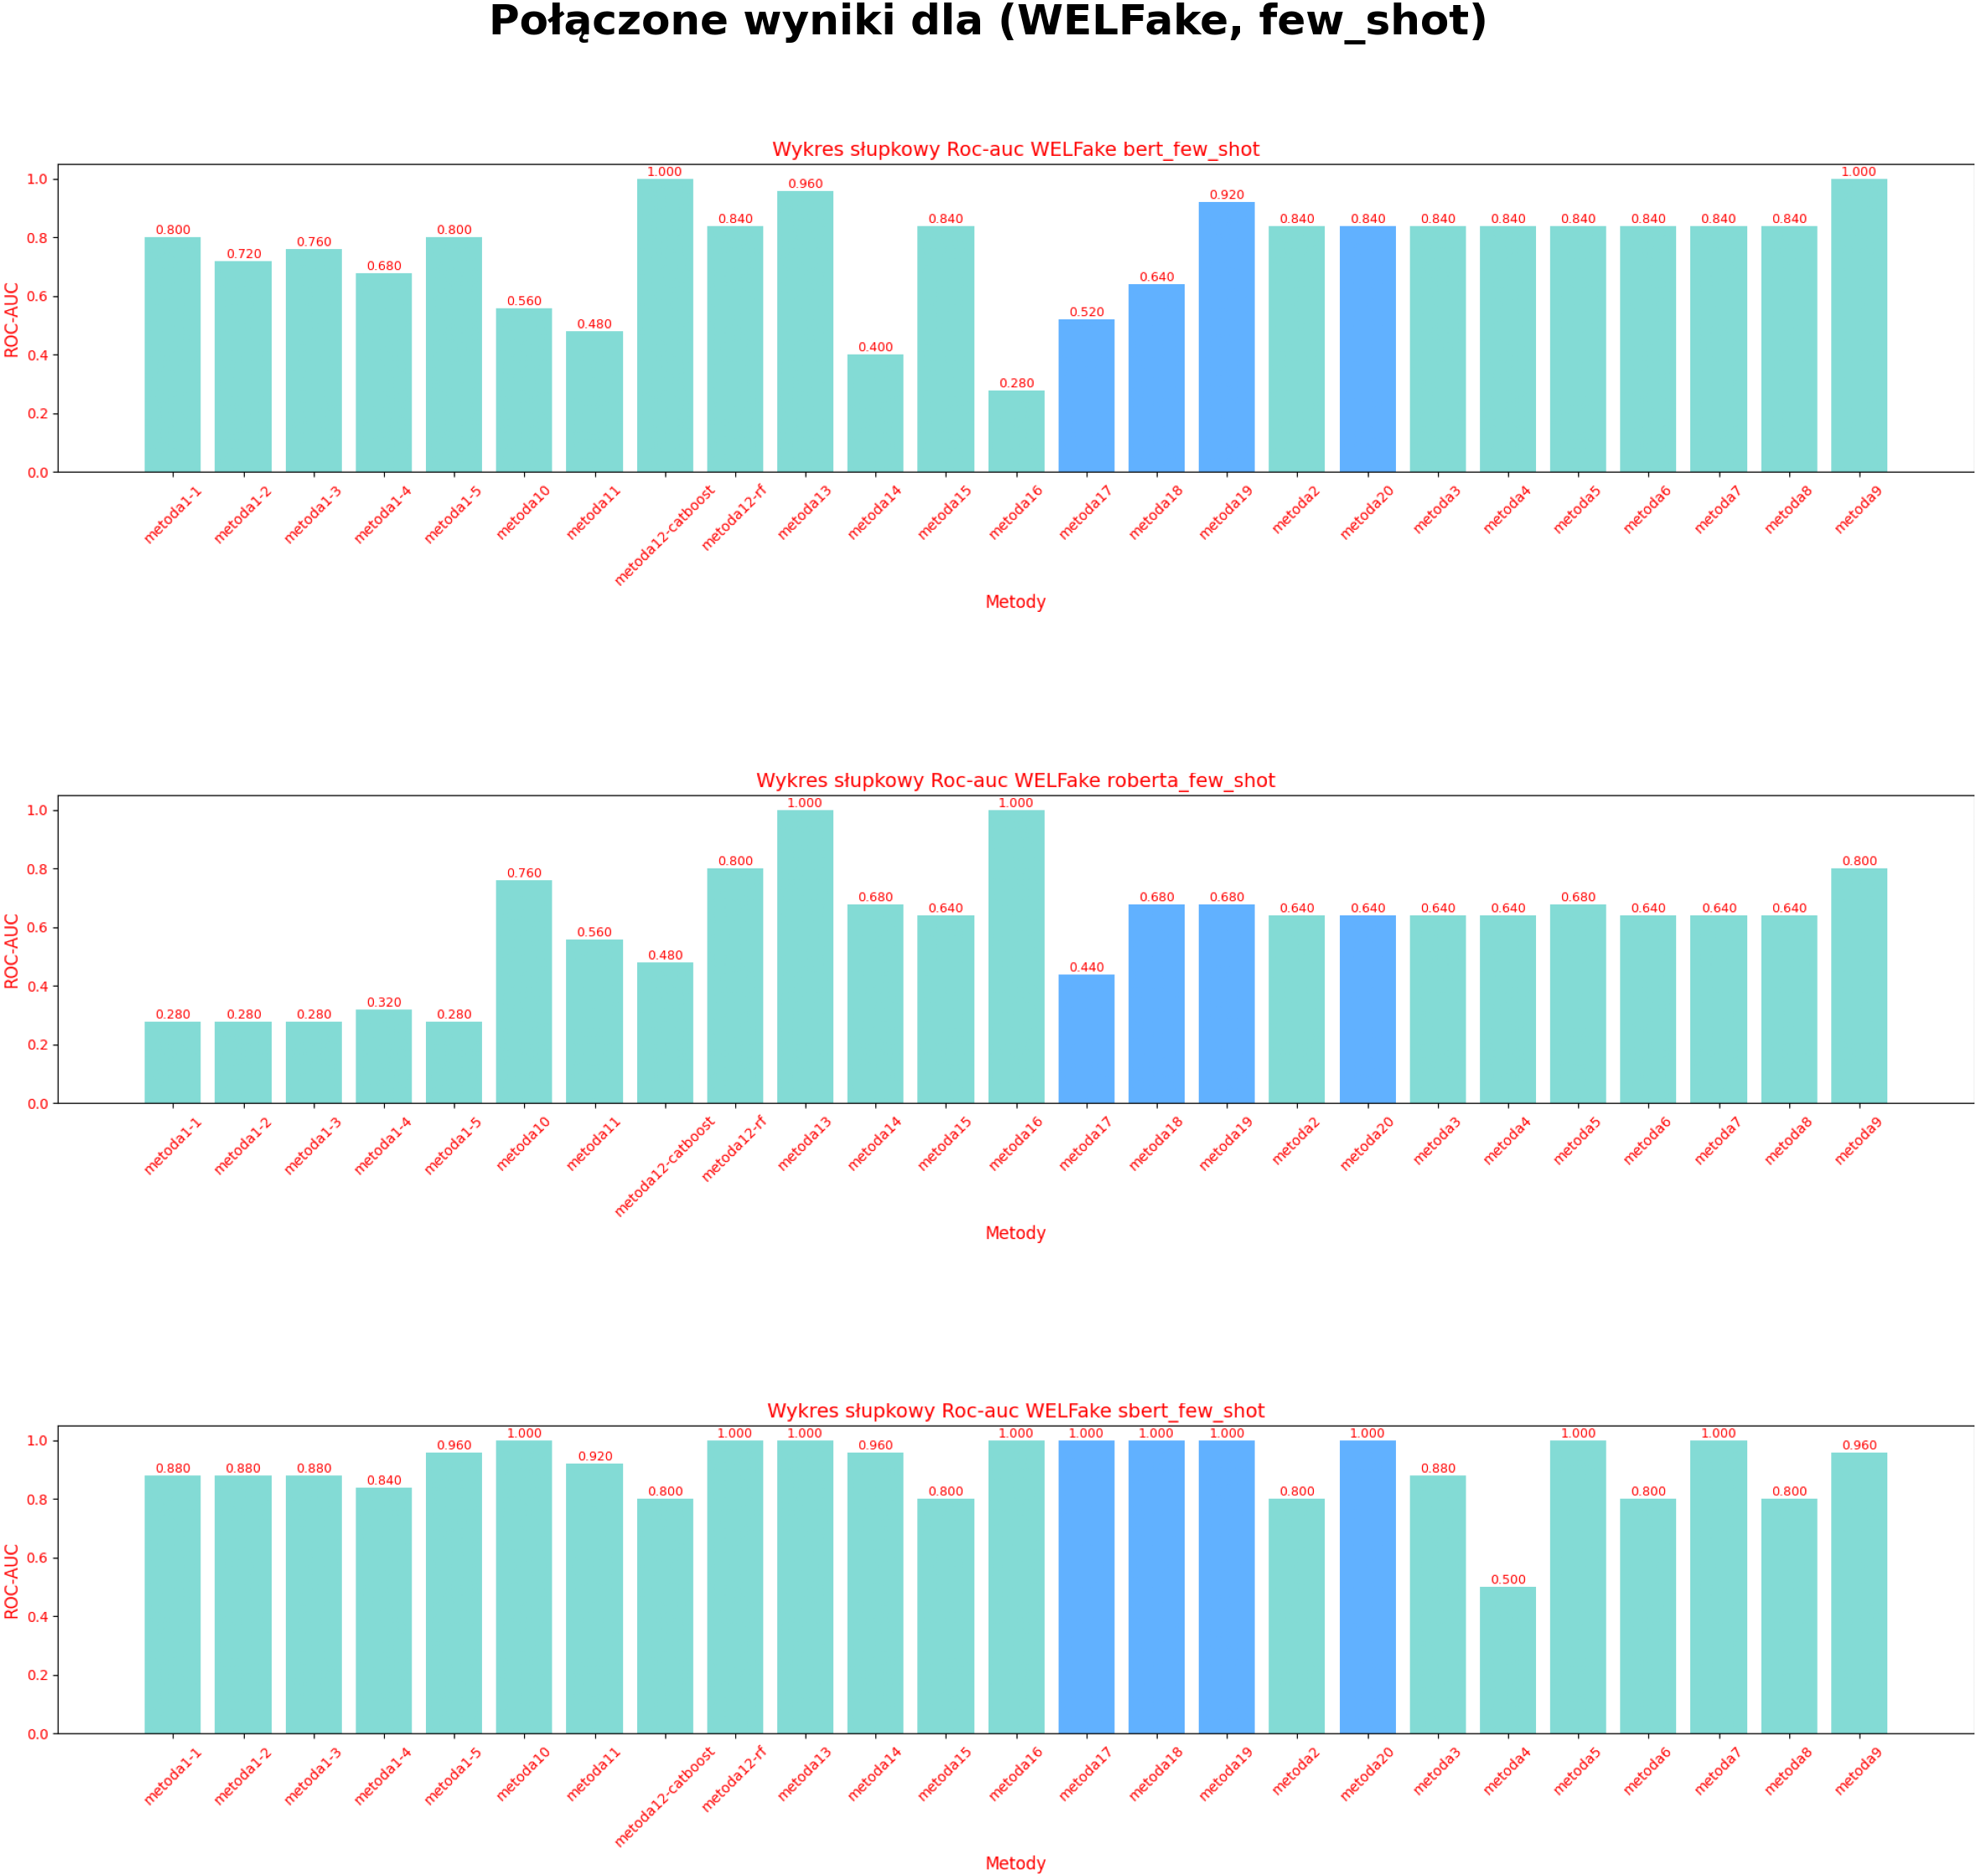
\includegraphics[width=0.99\textwidth]{img/stats/WELFake_few_shot/WELFake_few_shot_Combined_ROC-AUC_bar.png}
	\caption{Histogram rozkładu \textbf{Pola pod krzywą ROC-AUC (ROC-AUC)}.}
	\label{fig:welfake_few_shot_roc}
\end{figure}

\subsubsection{Czas wykonania}
Wykres liniowy \textbf{Czasu wykonania (Execution Time)} \ref{fig:welfake_few_shot_prcurve} przedstawia porównanie czasu potrzebnego na wykonanie predykcji. Na podstawie wykresów można sformułować następujące obserwacje:

\begin{itemize}
	\item \textbf{Wykres górny (BERT):}
	      \begin{itemize}
		      \item Najwięcej czasu, powyżej 500 sekund, zajęły \texttt{Metoda9} oraz \texttt{Metoda20}. \texttt{Metoda9} jest czasochłonna z powodu iteracyjnych algorytmów ensemble, a \texttt{Metoda20} z powodu trenowania LightGBM na dużych danych BERT.
		      \item Najkrótszy czas, poniżej 20 sekund, miały \texttt{Metoda18}, \texttt{Metoda7} oraz \texttt{Metoda10}, dzięki zoptymalizowanym modelom.
	      \end{itemize}

	\item \textbf{Wykres środkowy (RoBERTa):}
	      \begin{itemize}
		      \item Najwięcej czasu, od 200 do 500 sekund, zajęły \texttt{Metoda14}, \texttt{Metoda9} oraz \texttt{Metoda17}. \texttt{Metoda17} wymaga dodatkowego czasu na optymalizację VotingClassifiera.
		      \item Najkrótszy czas, poniżej 20 sekund, miały \texttt{Metoda18}, \texttt{Metoda7} oraz \texttt{Metoda10}.
	      \end{itemize}

	\item \textbf{Wykres dolny (SBERT):}
	      \begin{itemize}
		      \item Najdłuższy czas, około 2000 sekund, osiągnęła \texttt{Metoda4} z powodu złożonych warstw Bi-LSTM, CNN i MLP.
		      \item Najkrótszy czas, do 50 sekund, uzyskano dla \texttt{Metoda7} oraz \texttt{Metoda19}, dzięki prostym i zoptymalizowanym modelom.
	      \end{itemize}
\end{itemize}

Analiza czasów wykonania dla trybu few-shot pokazuje, że złożone modele, takie jak \texttt{Metoda4} czy \texttt{Metoda20}, są czasochłonne, podczas gdy \texttt{Metoda18} i \texttt{Metoda19} osiągają wysoką efektywność czasową, szczególnie dla SBERT.

\begin{figure}[H]
	\centering
	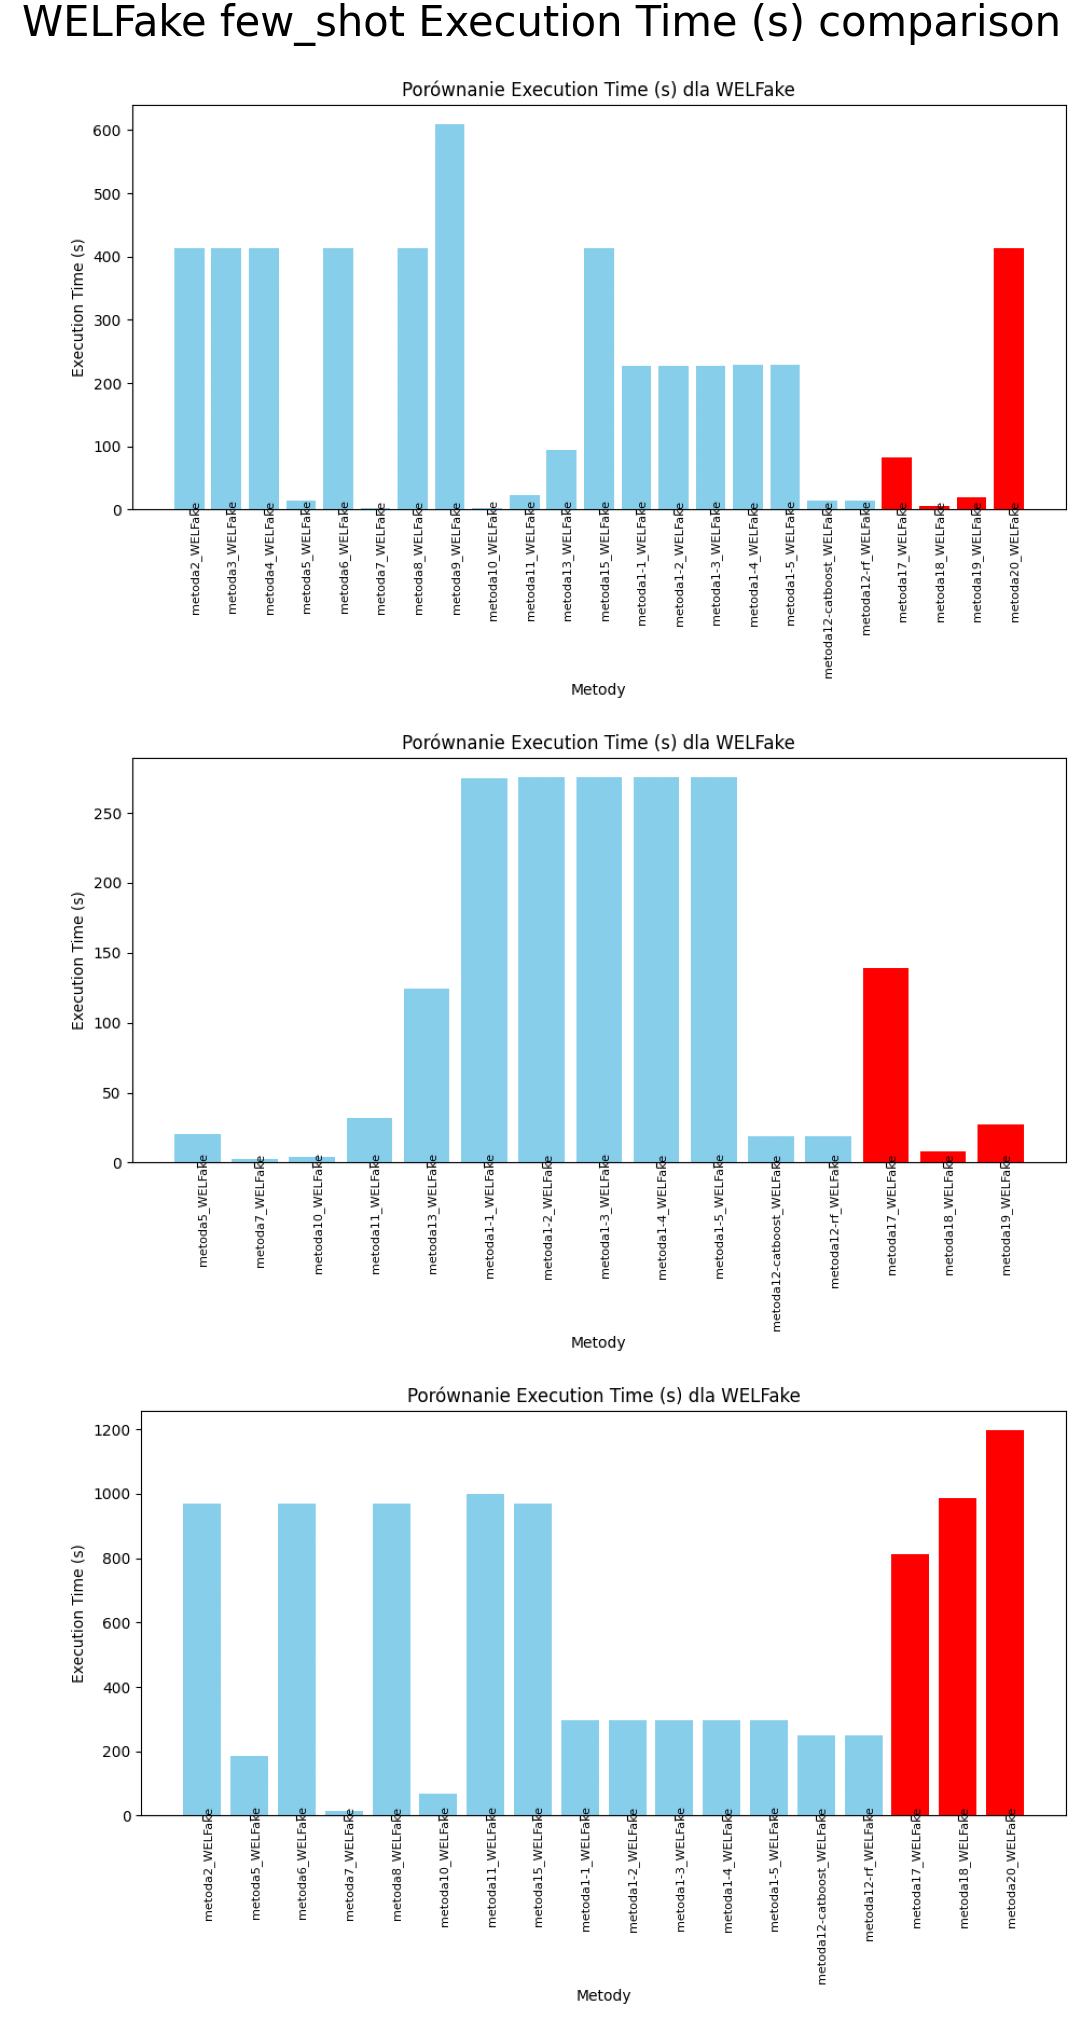
\includegraphics[width=0.99\textwidth]{img/stats/WELFake_few_shot/WELFake_few_shot_Execution Time (s)_comparison.png}
	\caption{\textbf{Czas wykonania (Execution Time)} w sekundach.}
	\label{fig:welfake_few_shot_prcurve}
\end{figure}

% Subsection for one-shot mode results
\subsection{Wyniki w trybie one-shot}

W trybie \textbf{one-shot} dla datasetu \textbf{WELFake} przetestowano metody klasyfikacji na pojedynczych przykładach treningowych. Poniżej przedstawiono szczegółowy opis wyników.

\subsubsection{Accuracy}
Wykresy słupkowe \textbf{Dokładności (Accuracy)} \ref{fig:welfake_one_shot_accuracy} przedstawiają rozkład wartości dokładności dla wszystkich metod. Na podstawie wykresów można sformułować następujące obserwacje:

\begin{itemize}
	\item \textbf{Wykres górny (BERT):}
	      \begin{itemize}
		      \item Większość metod osiągnęła dokładność około 1.0, co wskazuje na wysoką separowalność klas w danych BERT w trybie one-shot.
		      \item Najgorsze wyniki, około 0.5, odnotowano dla \texttt{Metoda17} oraz \texttt{Metoda11}. Słabe wyniki \texttt{Metoda17} mogą wynikać z nieoptymalnych wag VotingClassifiera.
	      \end{itemize}

	\item \textbf{Wykres środkowy (RoBERTa):}
	      \begin{itemize}
		      \item Wszystkie metody osiągnęły umiarkowaną dokładność, około 0.6, co wskazuje na trudności w generalizacji z pojedynczego przykładu dla RoBERTa.
		      \item Brak wyraźnych liderów sugeruje, że embeddingi RoBERTa są mniej separowalne w trybie one-shot.
	      \end{itemize}

	\item \textbf{Wykres dolny (SBERT):}
	      \begin{itemize}
		      \item Większość metod osiągnęła dokładność około 1.0, potwierdzając wysoką informatywność embeddingów SBERT.
		      \item Najgorsze wyniki, około 0.5, odnotowano dla \texttt{Metoda3}, \texttt{Metoda4}, \texttt{Metoda7}, \texttt{Metoda12-rf} oraz \texttt{Metoda19}. Słabe wyniki \texttt{Metoda19} mogą wynikać z braku optymalizacji ensemble.
	      \end{itemize}
\end{itemize}

Analiza dokładności dla trybu one-shot pokazuje, że BERT i SBERT umożliwiają perfekcyjne wyniki dla wielu metod, podczas gdy RoBERTa osiąga umiarkowane wyniki z powodu subtelniejszych reprezentacji.

\begin{figure}[H]
	\centering
	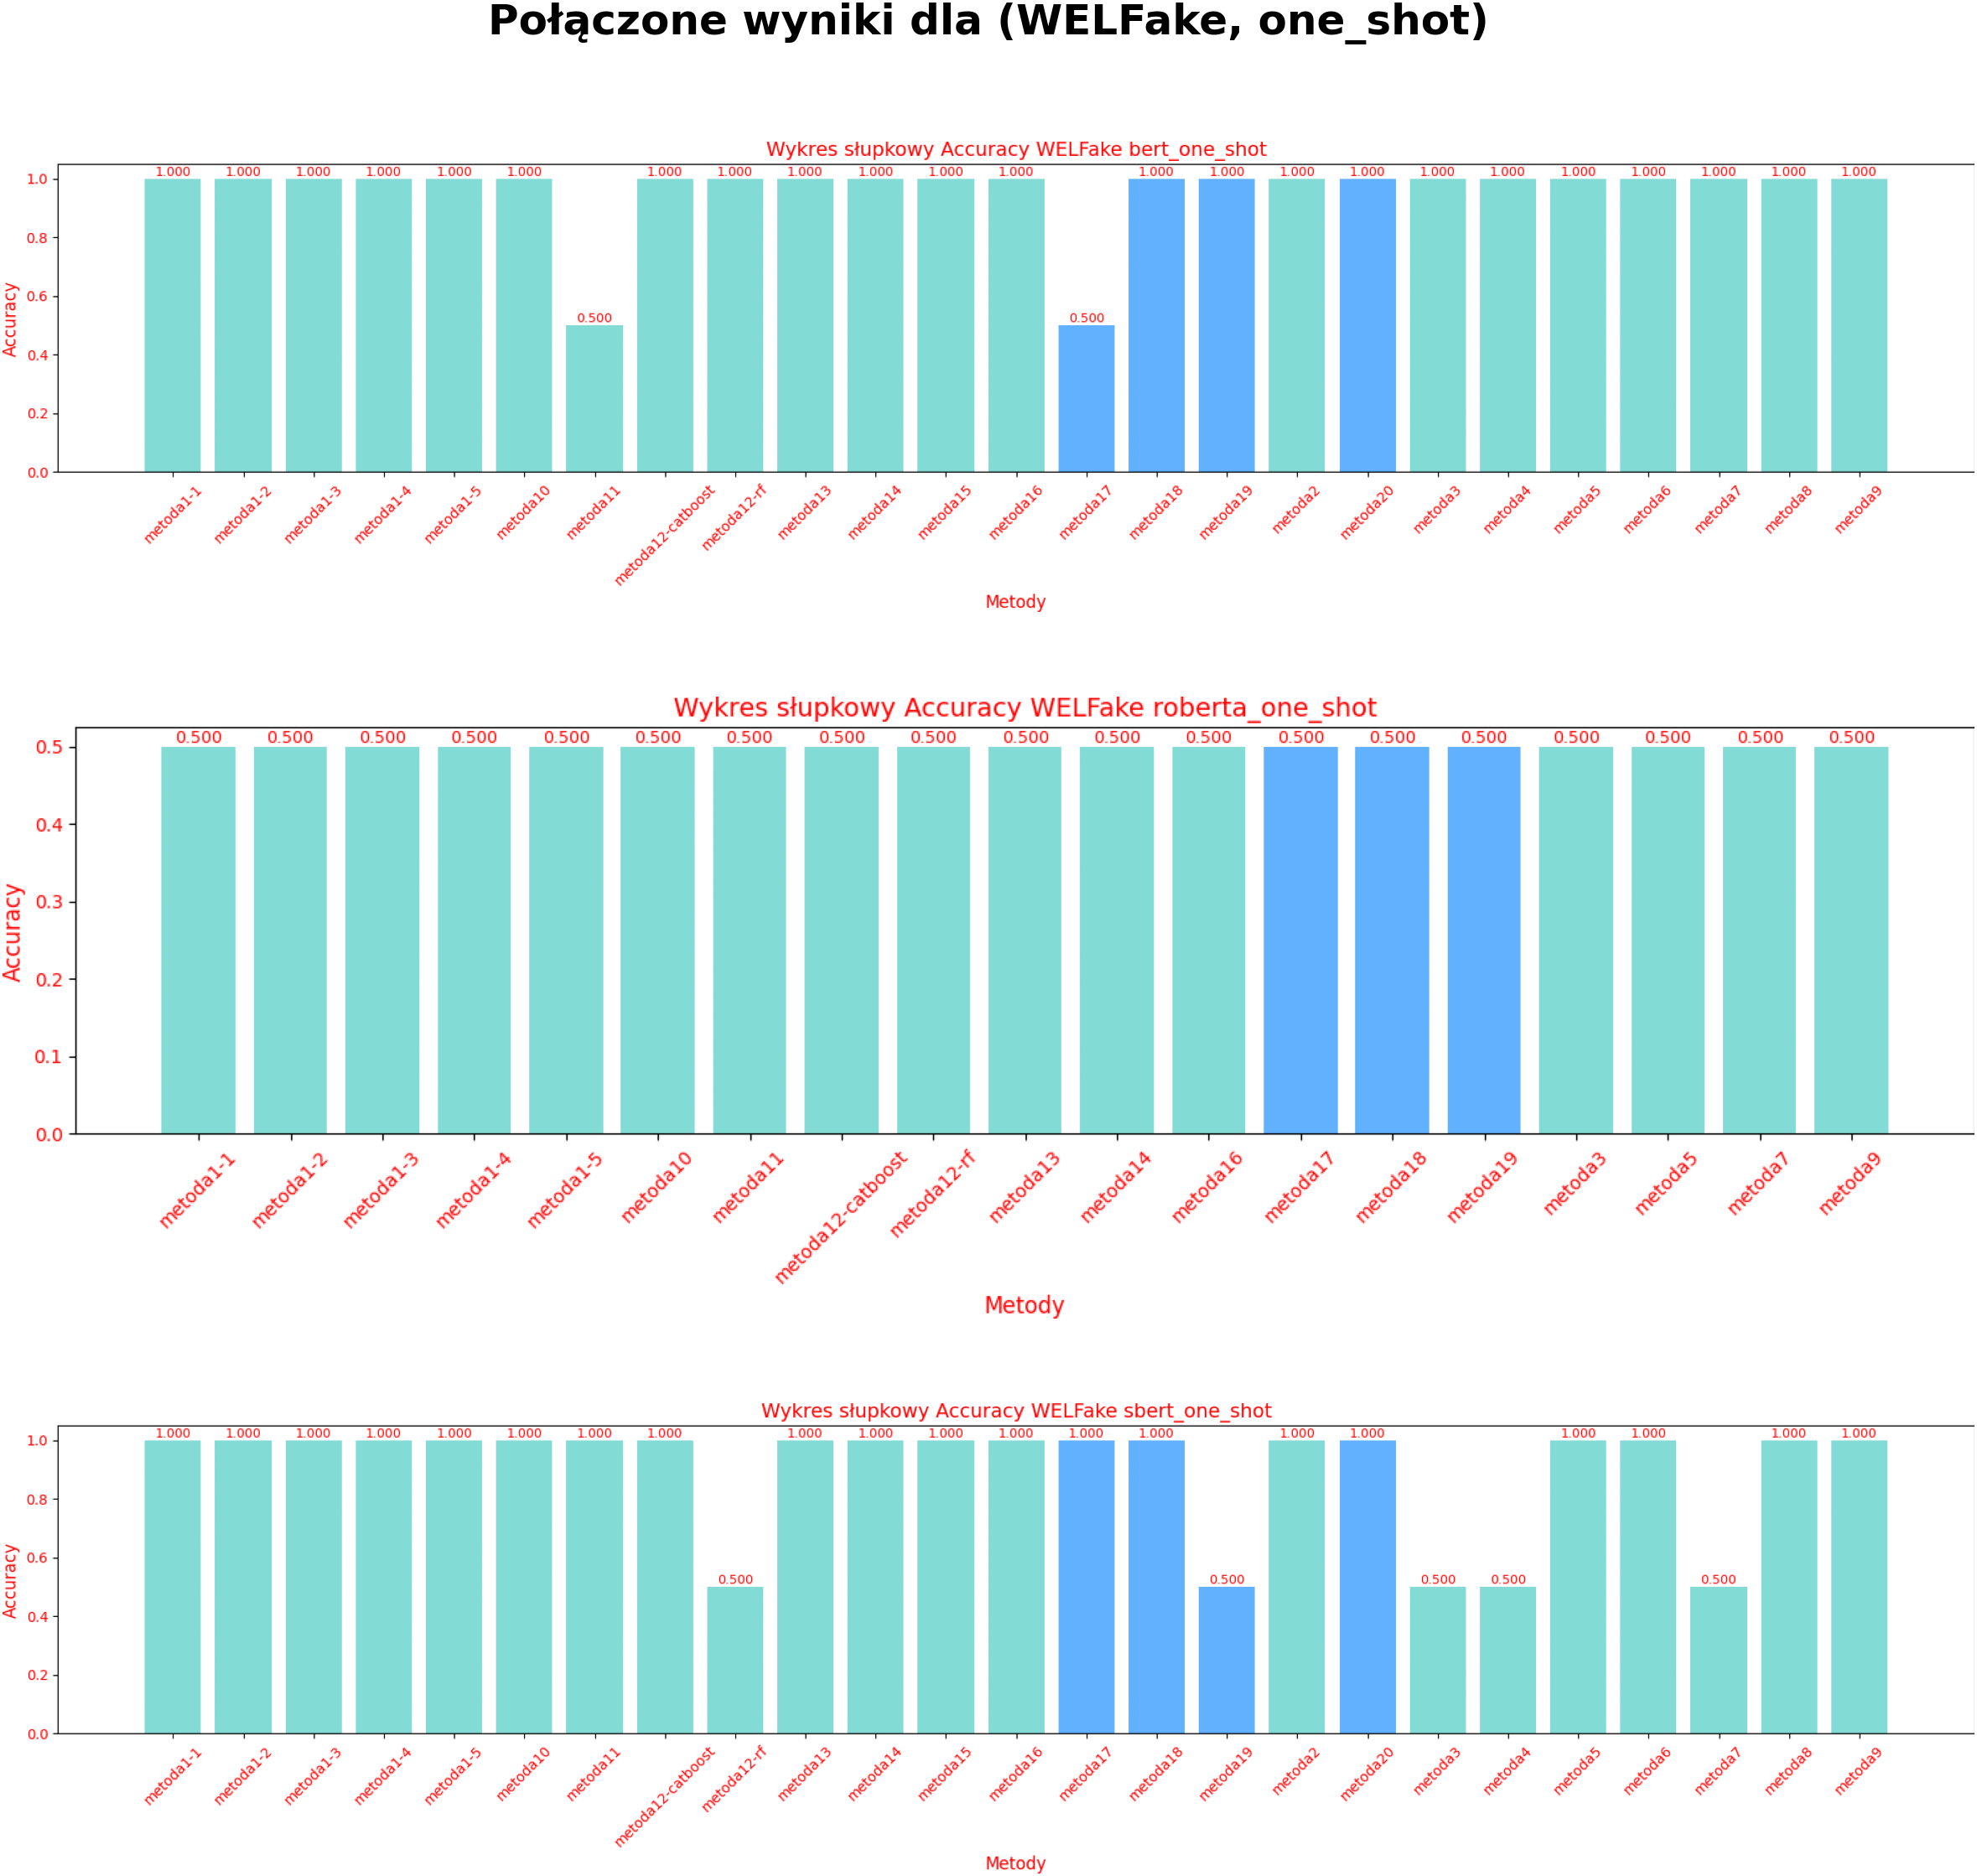
\includegraphics[width=0.99\textwidth]{img/stats/WELFake_one_shot/WELFake_one_shot_Combined_Accuracy_bar_chart.png}
	\caption{Histogram rozkładu \textbf{Dokładności (Accuracy)}.}
	\label{fig:welfake_one_shot_accuracy}
\end{figure}

\subsubsection{F1-Score}
Wykresy słupkowe \textbf{Wyniku F1 (F1-Score)} \ref{fig:welfake_one_shot_f1} przedstawiają rozkład wartości F1-Score dla wszystkich metod. Na podstawie wykresu można sformułować następujące obserwacje:

\begin{itemize}
	\item \textbf{Wykres górny (BERT):}
	      \begin{itemize}
		      \item Większość metod osiągnęła F1-Score około 1.0, co potwierdza wysoką separowalność klas w danych BERT.
		      \item Najniższe wyniki, około 0.5, odnotowano dla \texttt{Metoda17} oraz \texttt{Metoda11}. Słabe wyniki \texttt{Metoda17} mogą wynikać z niedopasowania VotingClassifiera.
	      \end{itemize}

	\item \textbf{Wykres środkowy (RoBERTa):}
	      \begin{itemize}
		      \item Większość metod osiągnęła F1-Score około 0.7, co wskazuje na trudności w trybie one-shot dla RoBERTa.
		      \item Najsłabsze wyniki, około 0.5, odnotowano dla \texttt{Metoda1-5}, \texttt{Metoda13} oraz \texttt{Metoda19}. Słabe wyniki \texttt{Metoda19} mogą wynikać z braku optymalizacji.
	      \end{itemize}

	\item \textbf{Wykres dolny (SBERT):}
	      \begin{itemize}
		      \item Większość metod osiągnęła F1-Score około 1.0, potwierdzając informatywność SBERT.
		      \item Najgorsze rezultaty, około 0.5, odnotowano dla \texttt{Metoda3}, \texttt{Metoda4}, \texttt{Metoda7}, \texttt{Metoda12-rf} oraz \texttt{Metoda19}. Słabe wyniki \texttt{Metoda19} wskazują na potrzebę lepszej optymalizacji.
	      \end{itemize}
\end{itemize}

Analiza F1-Score dla trybu one-shot potwierdza wysoką skuteczność BERT i SBERT, podczas gdy RoBERTa wymaga precyzyjniejszej optymalizacji.

\begin{figure}[H]
	\centering
	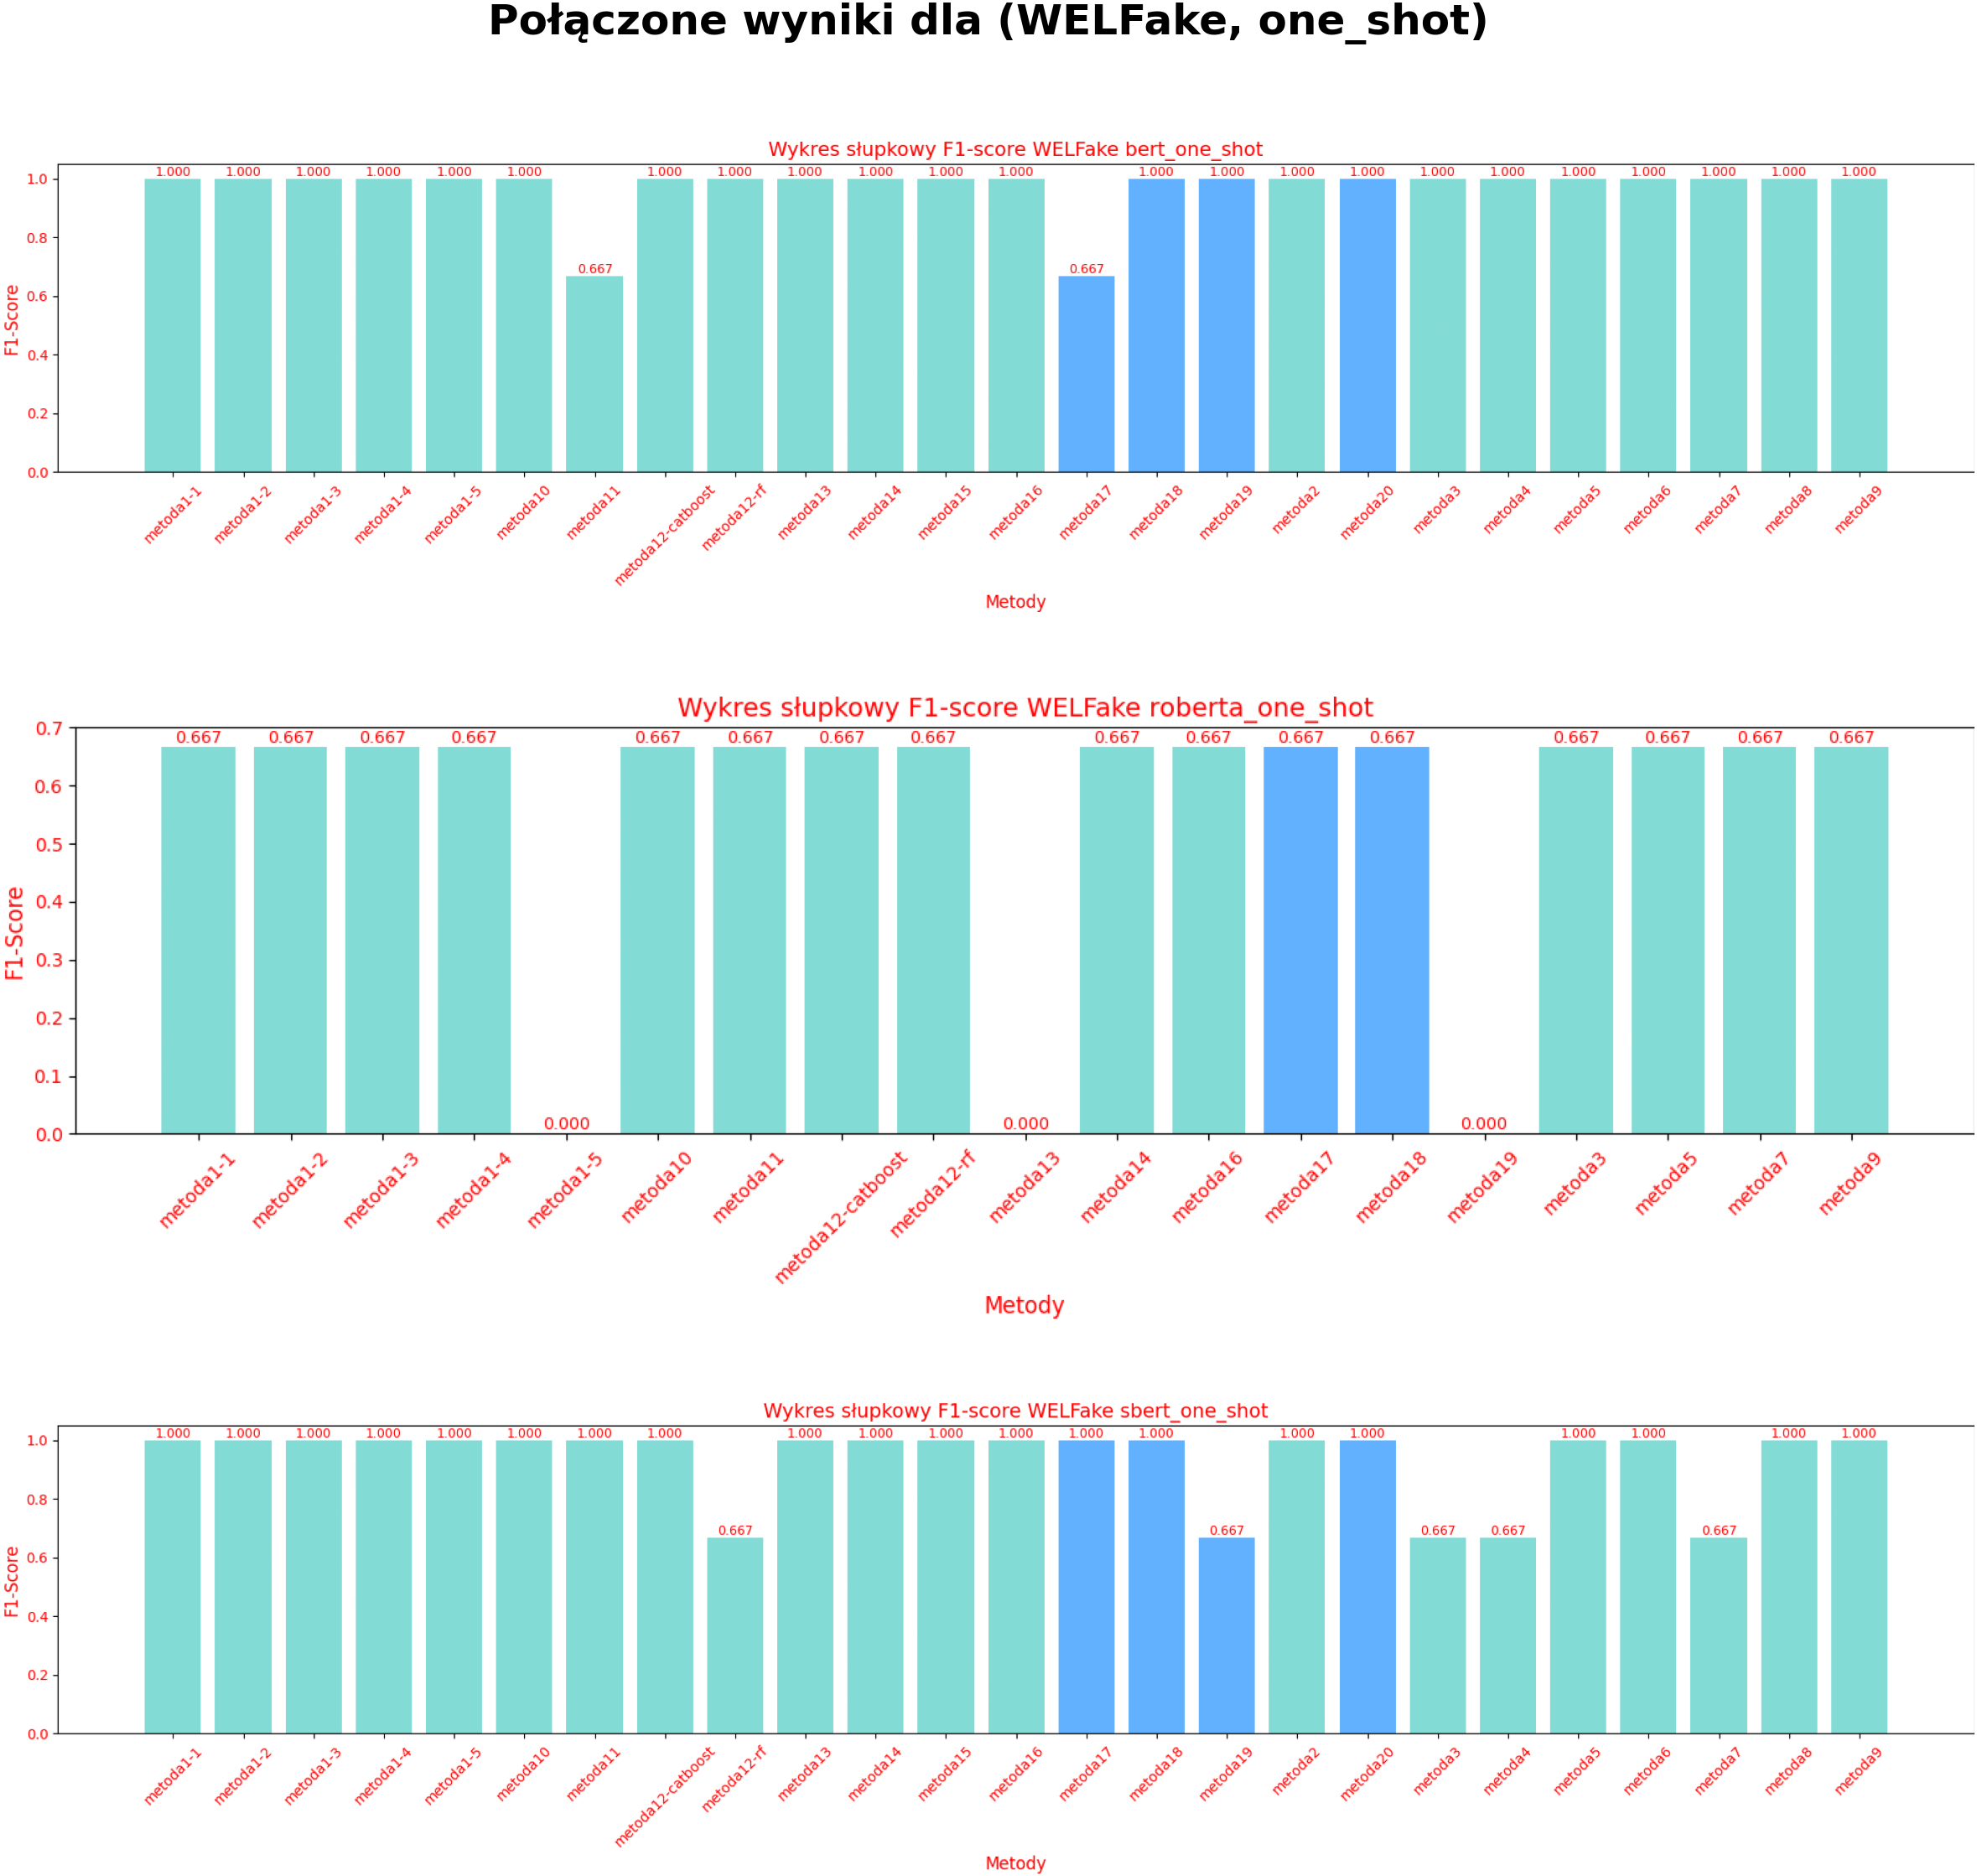
\includegraphics[width=0.99\textwidth]{img/stats/WELFake_one_shot/WELFake_one_shot_Combined_F1-Score_bar.png}
	\caption{Histogram rozkładu \textbf{Wyniku F1 (F1-Score)}.}
	\label{fig:welfake_one_shot_f1}
\end{figure}

\subsubsection{ROC-AUC}
Wykresy słupkowe \textbf{Pola pod krzywą ROC-AUC (ROC-AUC)} \ref{fig:welfake_one_shot_roc} przedstawiają rozkład wartości ROC-AUC dla wszystkich metod. Na podstawie wykresu można sformułować następujące obserwacje:

\begin{itemize}
	\item \textbf{Wykres górny (BERT):}
	      \begin{itemize}
		      \item Wszystkie metody osiągnęły ROC-AUC około 1.0, co potwierdza doskonałą separowalność klas w danych BERT.
	      \end{itemize}

	\item \textbf{Wykres środkowy (RoBERTa):}
	      \begin{itemize}
		      \item Najlepsze wartości ROC-AUC, około 0.9, osiągnęły \texttt{Metoda12-rf}, \texttt{Metoda13}, \texttt{Metoda17} oraz \texttt{Metoda18}. Wysoka skuteczność wskazuje na zdolność tych metod do rozróżniania klas.
		      \item Najsłabsze wyniki, około 0.6, odnotowano dla pozostałych metod, w tym \texttt{Metoda19}. Słabe wyniki \texttt{Metoda19} mogą wynikać z braku optymalizacji.
	      \end{itemize}

	\item \textbf{Wykres dolny (SBERT):}
	      \begin{itemize}
		      \item Większość metod osiągnęła ROC-AUC około 1.0, potwierdzając informatywność SBERT.
		      \item Słabe rezultaty, około 0.5, odnotowano dla \texttt{Metoda4}. Niska wartość ROC-AUC może wynikać z trudności w optymalizacji złożonej architektury.
	      \end{itemize}
\end{itemize}

Analiza ROC-AUC dla trybu one-shot pokazuje, że BERT i SBERT umożliwiają perfekcyjne wyniki, podczas gdy RoBERTa wymaga lepszej optymalizacji dla niektórych metod, takich jak \texttt{Metoda19}.

\begin{figure}[H]
	\centering
	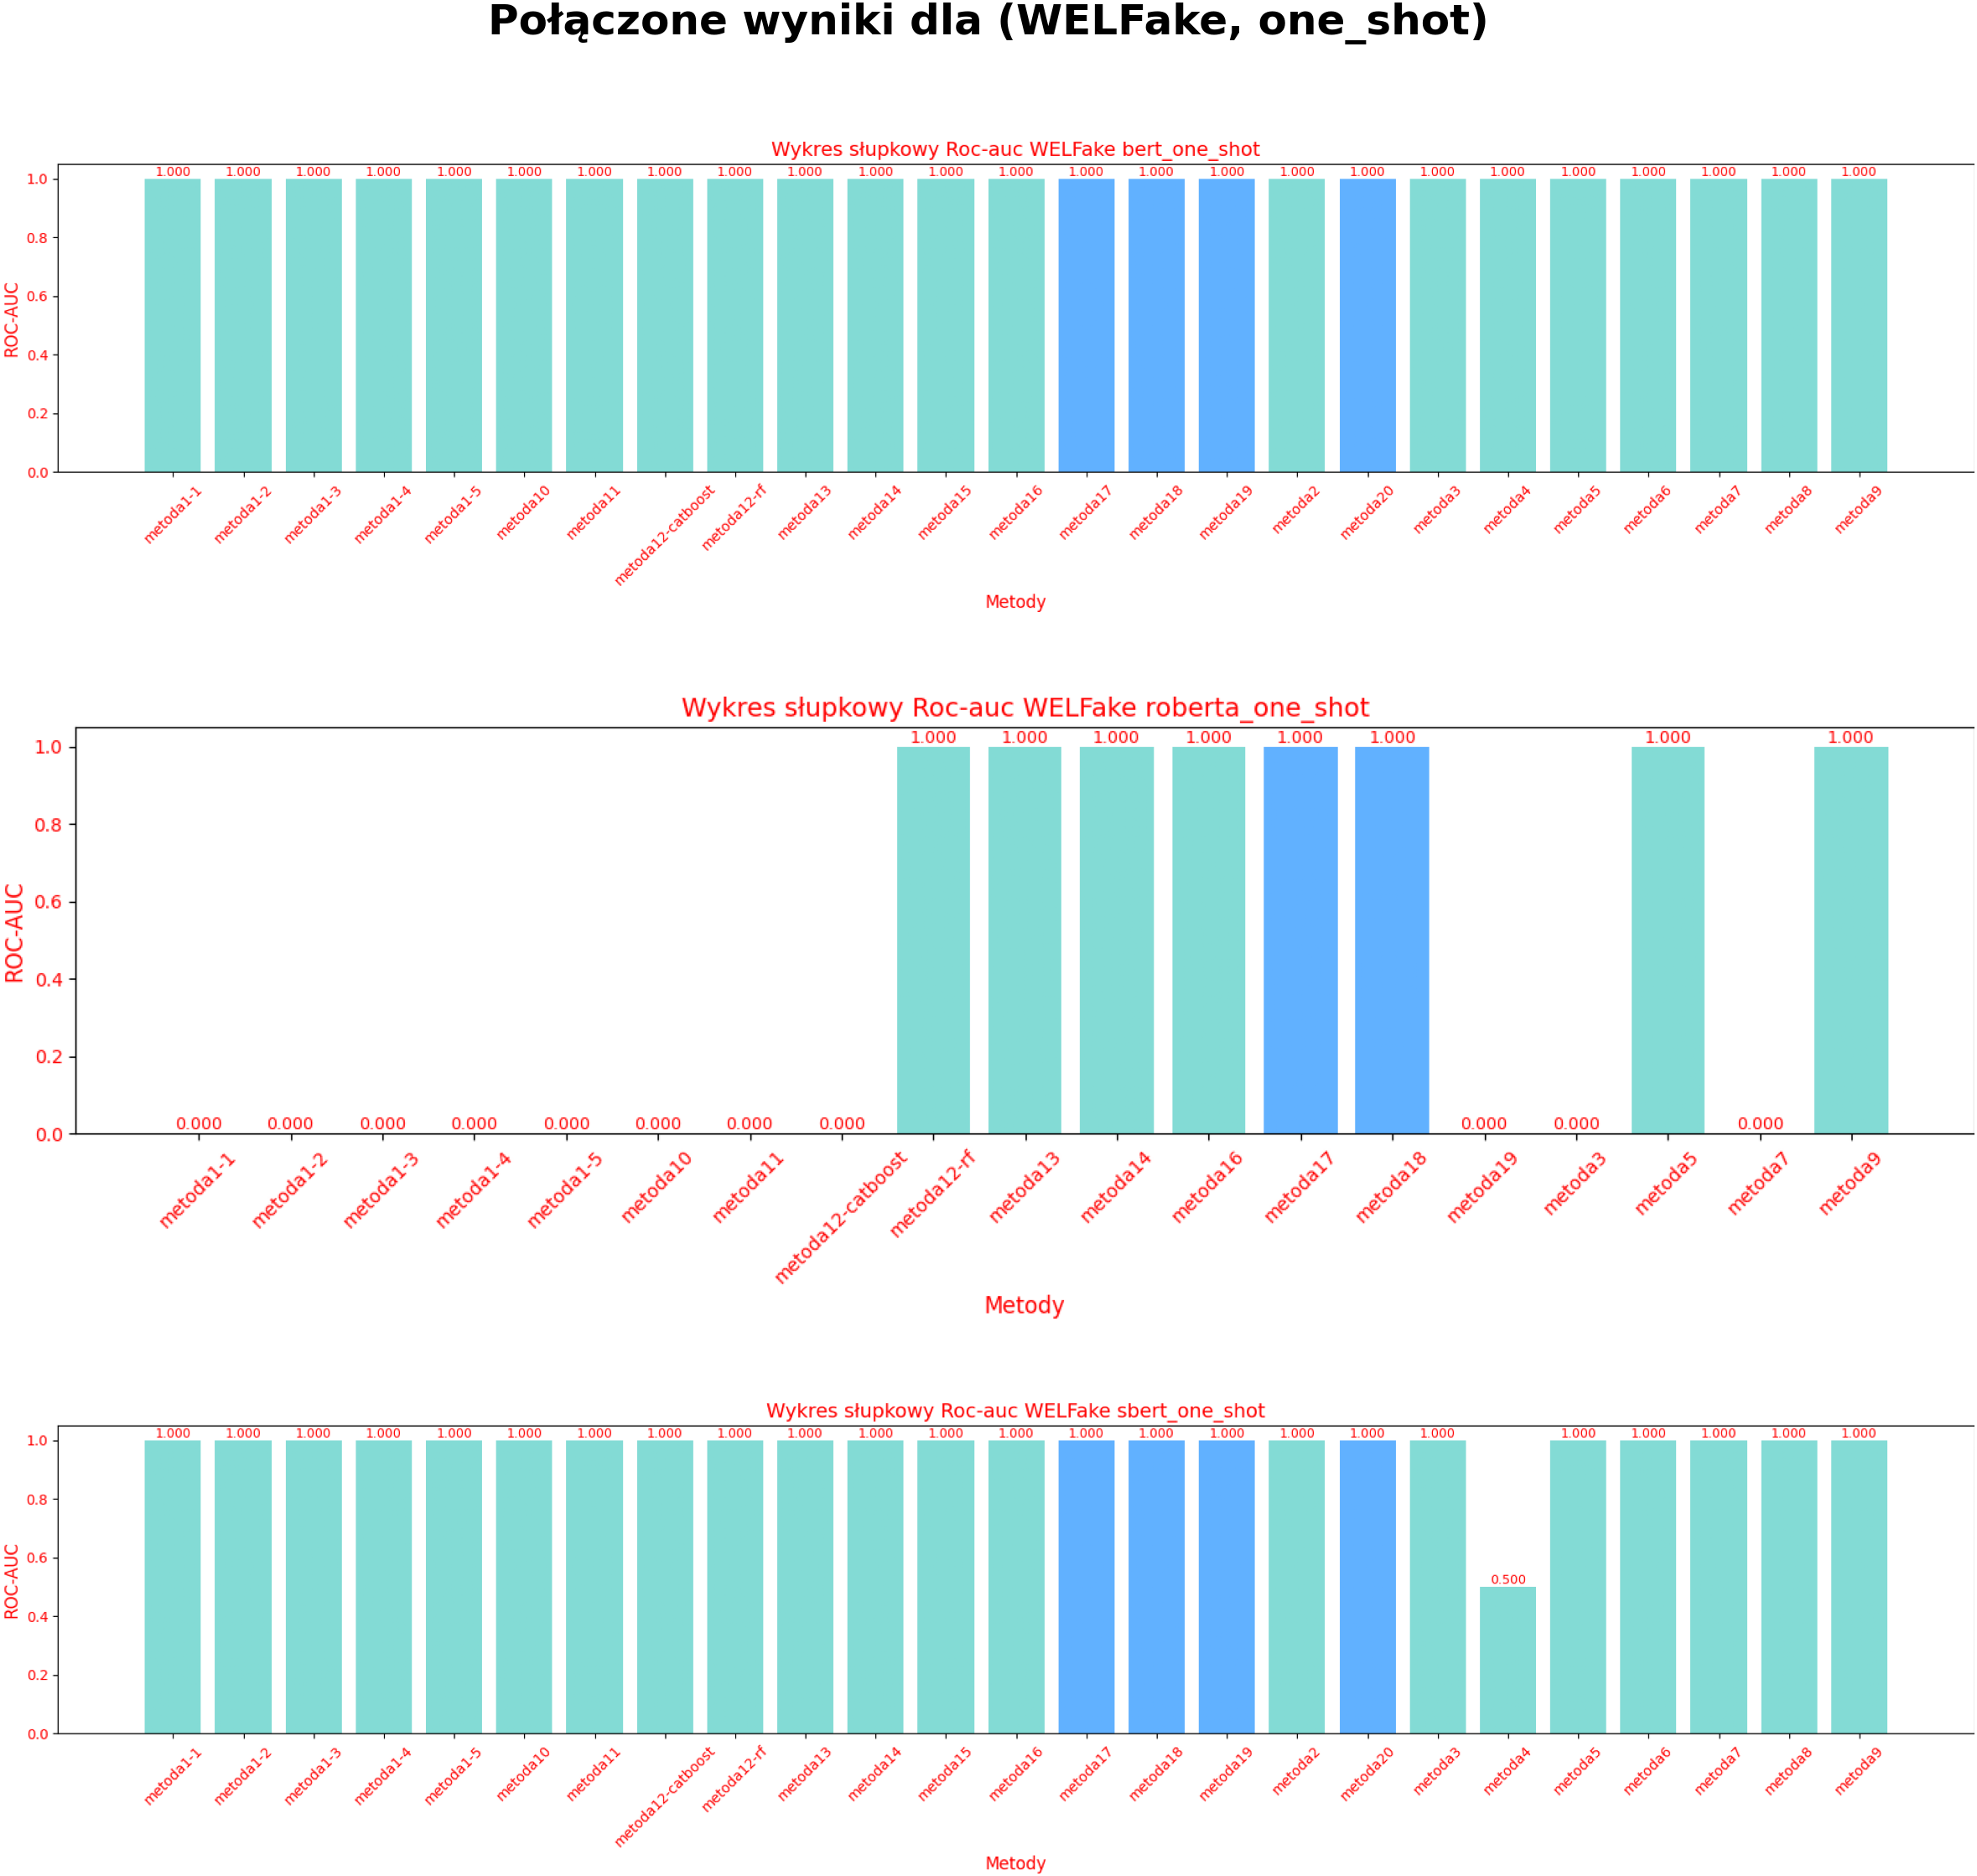
\includegraphics[width=0.99\textwidth]{img/stats/WELFake_one_shot/WELFake_one_shot_Combined_ROC-AUC_bar.png}
	\caption{Histogram rozkładu \textbf{Pola pod krzywą ROC-AUC (ROC-AUC)}.}
	\label{fig:welfake_one_shot_roc}
\end{figure}

\subsubsection{Czas wykonania}
Wykres liniowy \textbf{Czasu wykonania (Execution Time)} \ref{fig:welfake_one_shot_prcurve} przedstawia porównanie czasu potrzebnego na wykonanie predykcji. Na podstawie wykresów można sformułować następujące obserwacje:

\begin{itemize}
	\item \textbf{Wykres górny (BERT):}
	      \begin{itemize}
		      \item Najdłuższy czas, około 140 sekund, odnotowano dla \texttt{Metoda2}, \texttt{Metoda3}, \texttt{Metoda4}, \texttt{Metoda8}, \texttt{Metoda15} oraz \texttt{Metoda20}. \texttt{Metoda20} jest czasochłonna z powodu trenowania LightGBM na dużych danych.
		      \item Najkrótszy czas, poniżej 10 sekund, miały \texttt{Metoda7}, \texttt{Metoda10} oraz \texttt{Metoda18}.
	      \end{itemize}

	\item \textbf{Wykres środkowy (RoBERTa):}
	      \begin{itemize}
		      \item Najwięcej czasu, około 400 sekund, zajęła \texttt{Metoda9} z powodu iteracyjnych algorytmów ensemble.
		      \item Najkrótszy czas, poniżej 5 sekund, miały \texttt{Metoda7}, \texttt{Metoda18} oraz \texttt{Metoda19}.
	      \end{itemize}

	\item \textbf{Wykres dolny (SBERT):}
	      \begin{itemize}
		      \item Najdłuższy czas, przekraczający 1200 sekund, osiągnęła \texttt{Metoda3} z powodu złożonej architektury ensemble.
		      \item Najkrótszy czas, w okolicach 100 sekund, uzyskano dla \texttt{Metoda7}, \texttt{Metoda17} oraz \texttt{Metoda19}.
	      \end{itemize}
\end{itemize}

Analiza czasów wykonania dla trybu one-shot pokazuje, że złożone modele, takie jak \texttt{Metoda3} czy \texttt{Metoda20}, są czasochłonne, podczas gdy \texttt{Metoda18} i \texttt{Metoda19} osiągają wysoką efektywność czasową.

\begin{figure}[H]
	\centering
	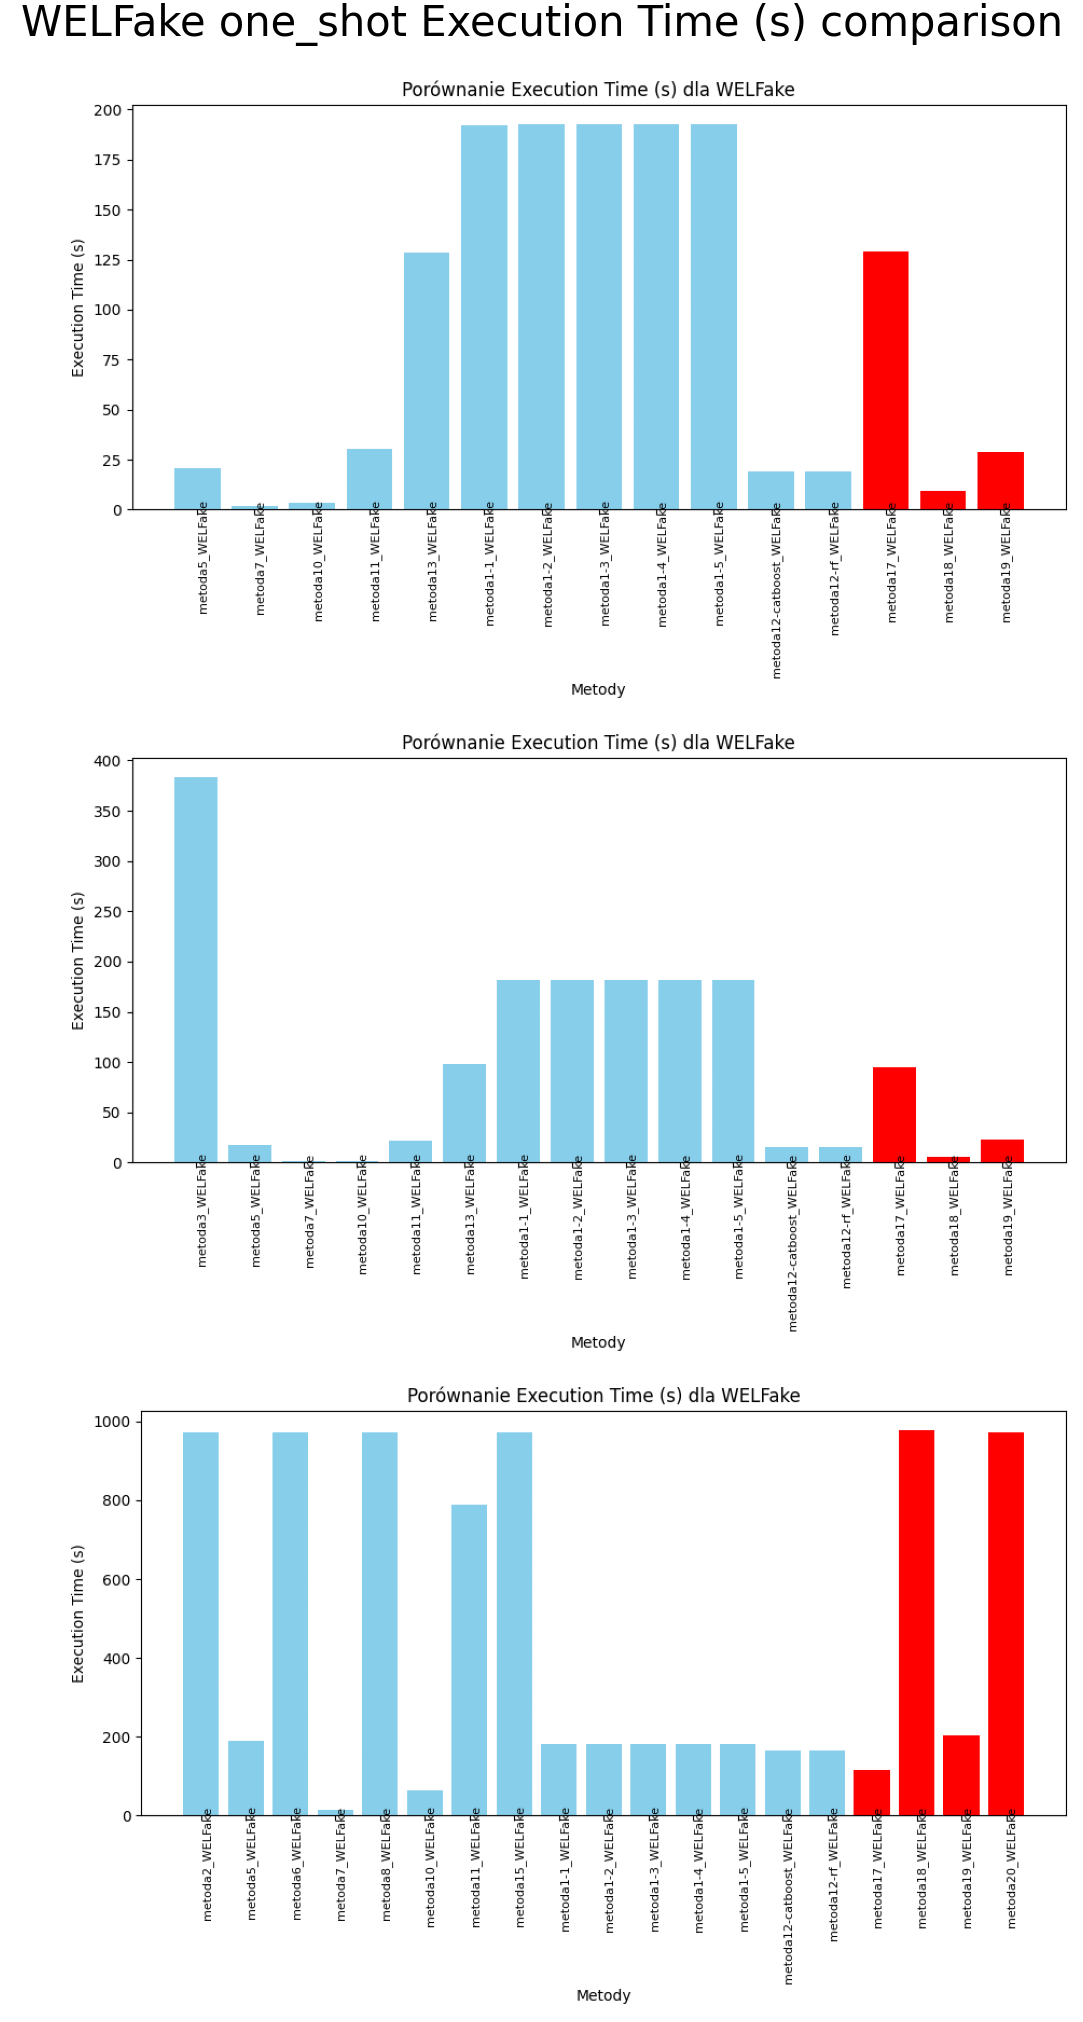
\includegraphics[width=0.99\textwidth]{img/stats/WELFake_one_shot/WELFake_one_shot_Execution Time (s)_comparison.png}
	\caption{\textbf{Czas wykonania (Execution Time)} w sekundach.}
	\label{fig:welfake_one_shot_prcurve}
\end{figure}

% Subsection for additional analysis
\subsection{Dodatkowa analiza wyników dla datasetu WELFake}
\label{subsec:welfake_additional_analysis}

W tej podsekcji przedstawiono szczegółową analizę wyników dla datasetu \textbf{WELFake}, obejmującą wyniki AUC-PR, testy normalności rozkładów, macierze korelacji Pearsona i Spearmana oraz testy statystyczne Kruskal-Wallis. Analiza ma na celu ocenę wydajności wszystkich metod oraz uzasadnienie sensu stosowania bardziej złożonych metod autorskich (\texttt{Metoda17}, \texttt{Metoda18}, \texttt{Metoda19}, \texttt{Metoda20}) w kontekście ich zalet w różnych scenariuszach uczenia.

\subsubsection{Wyniki AUC-PR}
Tabela \ref{tab:welfake_auc_pr} przedstawia wyniki AUC-PR dla różnych metod. Najwyższy wynik, 0.9556, osiągnęła \texttt{Metoda13}. Wśród metod autorskich \texttt{Metoda18} osiągnęła 0.8932, \texttt{Metoda20} 0.8863, \texttt{Metoda17} 0.8469, a \texttt{Metoda19} 0.8266. \texttt{Metoda17} osiąga średnie wyniki z powodu nieoptymalnych wag VotingClassifiera. \texttt{Metoda18} jest skuteczna dzięki stackingowi z CatBoost. \texttt{Metoda19} ma słabsze wyniki z powodu braku balansowania klas. \texttt{Metoda20} osiąga dobre wyniki dzięki zoptymalizowanemu LightGBM.

\begin{table}[H]
	\centering
	\caption{Wyniki AUC-PR dla metod na datasecie WELFake}
	\label{tab:welfake_auc_pr}
	\begin{tabular}{l r}
		\toprule
		Metoda                     & AUC-PR \\
		\midrule
		\texttt{metoda13}          & 0.9556 \\
		\texttt{metoda12-rf}       & 0.9248 \\
		\texttt{metoda9}           & 0.9207 \\
		\texttt{metoda5}           & 0.8982 \\
		\texttt{metoda14}          & 0.8955 \\
		\texttt{metoda18}          & 0.8932 \\
		\texttt{metoda16}          & 0.8923 \\
		\texttt{metoda20}          & 0.8863 \\
		\texttt{metoda2}           & 0.8633 \\
		\texttt{metoda8}           & 0.8633 \\
		\texttt{metoda15}          & 0.8633 \\
		\texttt{metoda6}           & 0.8633 \\
		\texttt{metoda17}          & 0.8469 \\
		\texttt{metoda19}          & 0.8266 \\
		\texttt{metoda10}          & 0.8126 \\
		\texttt{metoda7}           & 0.8111 \\
		\texttt{metoda12-catboost} & 0.8109 \\
		\texttt{metoda4}           & 0.8054 \\
		\texttt{metoda3}           & 0.7989 \\
		\texttt{metoda11}          & 0.7912 \\
		\texttt{metoda1-5}         & 0.7730 \\
		\texttt{metoda1-1}         & 0.7623 \\
		\texttt{metoda1-3}         & 0.7579 \\
		\texttt{metoda1-2}         & 0.7575 \\
		\texttt{metoda1-4}         & 0.7527 \\
		\bottomrule
	\end{tabular}
\end{table}

\subsubsection{Testy normalności i analizy statystyczne}
Testy Shapiro-Wilka wykazały, że większość metryk (Accuracy, Precision, Recall, F1-Score, ROC-AUC, MCC, Cohen’s Kappa, AUC-PR) ma rozkład normalny (p-value > 0.05), z wyjątkiem Accuracy dla \texttt{Metoda17} (p-value = 0.0065). Testy Kruskal-Wallisa nie wykazały istotnych statystycznych różnic między metodami (p-value > 0.05), z najwyższym p-value dla F1-Score (0.9669). Wynik ten sugeruje, że prostsze metody, takie jak \texttt{Metoda9}, mogą być równie skuteczne jak bardziej złożone metody autorskie w trybie klasycznym, ale złożone metody oferują przewagę w trudniejszych scenariuszach, takich jak few-shot i one-shot.

\subsubsection{Analiza korelacji}
Macierze korelacji Pearsona i Spearmana ujawniły silne dodatnie zależności między metrykami. Najsilniejsze korelacje w macierzy Pearsona zaobserwowano między Accuracy a Cohen’s Kappa (0.9990), Accuracy a MCC (0.9972) oraz ROC-AUC a AUC-PR (0.9689). W macierzy Spearmana korelacje te wynoszą odpowiednio 0.9900, 0.9815 oraz 0.9691. Brak silnych ujemnych korelacji wskazuje na zgodność metryk w ocenie wydajności modeli.

\begin{table}[H]
	\centering
	\caption{Kluczowe współczynniki korelacji Pearsona}
	\label{tab:welfake_pearson_correlations}
	\begin{tabular}{l r l}
		\toprule
		Para metryk               & Współczynnik Pearsona & Interpretacja         \\
		\midrule
		Accuracy -- Cohen’s Kappa & 0.9990                & Bardzo silna dodatnia \\
		Accuracy -- MCC           & 0.9972                & Bardzo silna dodatnia \\
		MCC -- Cohen’s Kappa      & 0.9969                & Bardzo silna dodatnia \\
		Precision -- F1-Score     & 0.7951                & Silna dodatnia        \\
		Recall -- F1-Score        & 0.5878                & Umiarkowana dodatnia  \\
		ROC-AUC -- AUC-PR         & 0.9689                & Bardzo silna dodatnia \\
		\bottomrule
	\end{tabular}
\end{table}

\begin{table}[H]
	\centering
	\caption{Kluczowe współczynniki korelacji Spearmana}
	\label{tab:welfake_spearman_correlations}
	\begin{tabular}{l r l}
		\toprule
		Para metryk               & Współczynnik Spearmana & Interpretacja         \\
		\midrule
		Accuracy -- Cohen’s Kappa & 0.9900                 & Bardzo silna dodatnia \\
		Accuracy -- MCC           & 0.9815                 & Bardzo silna dodatnia \\
		MCC -- Cohen’s Kappa      & 0.9707                 & Bardzo silna dodatnia \\
		Precision -- F1-Score     & 0.6672                 & Silna dodatnia        \\
		Recall -- F1-Score        & 0.5145                 & Umiarkowana dodatnia  \\
		ROC-AUC -- AUC-PR         & 0.9691                 & Bardzo silna dodatnia \\
		\bottomrule
	\end{tabular}
\end{table}

% Subsection for conclusions
\subsection{Podsumowanie wniosków}
Analiza wyników dla datasetu \textbf{WELFake} pokazuje, że zaawansowane modele ensemble, takie jak \texttt{Metoda12-rf}, \texttt{Metoda13}, \texttt{Metoda18} oraz \texttt{Metoda19}, osiągają wysoką skuteczność w trybach klasycznym, few-shot i one-shot, szczególnie dla embeddingów \textbf{SBERT}. W trybie one-shot \textbf{BERT} i \textbf{SBERT} umożliwiają perfekcyjne wyniki (około 100\% Accuracy i F1-Score) dla wielu metod, co świadczy o ich zdolności do generowania wysoce separowalnych reprezentacji. \textbf{RoBERTa} osiąga umiarkowane wyniki (60–70\%) w trybie one-shot z powodu subtelniejszych reprezentacji, które wymagają precyzyjniejszej optymalizacji.

\begin{itemize}
	\item \textbf{Metoda17} (VotingClassifier) jest skuteczna dla \textbf{SBERT} w trybach klasycznym i few-shot dzięki elastyczności VotingClassifiera, ale słaba dla \textbf{BERT} i \textbf{RoBERTa} z powodu nieoptymalnych wag głosowania, co ogranicza jej zdolność do generalizacji.
	\item \textbf{Metoda18} (stacking z CatBoost) dominuje dla \textbf{SBERT} w trybach klasycznym i few-shot dzięki zoptymalizowanemu łączeniu modeli bazowych, ale osiąga słabsze wyniki dla \textbf{RoBERTa} w trybie one-shot z powodu zbyt prostej konfiguracji meta-klasyfikatora.
	\item \textbf{Metoda19} (stacking) osiąga wysokie wyniki dla \textbf{BERT} i \textbf{RoBERTa} w trybach klasycznym i few-shot dzięki zoptymalizowanemu ensemble, ale jest słaba dla \textbf{SBERT} w trybie one-shot z powodu braku odpowiedniego balansowania klas.
	\item \textbf{Metoda20} (LightGBM) jest skuteczna dla \textbf{BERT} i \textbf{SBERT} w trybie one-shot dzięki zoptymalizowanym modelom, ale osiąga średnie wyniki w innych trybach z powodu braku balansowania klas.
	\item Prostsze modele, takie jak \texttt{Metoda1-x}, osiągają zróżnicowane wyniki, z dobrymi rezultatami dla \textbf{SBERT}, ale słabszymi dla \textbf{RoBERTa}, co wskazuje na ich ograniczenia w trudniejszych scenariuszach.
\end{itemize}

Wysoka separowalność klas w datasecie \textbf{WELFake} ułatwia klasyfikację dla zoptymalizowanych metod, takich jak \texttt{Metoda18} i \texttt{Metoda19}, ale wymaga precyzyjnej konfiguracji hiperparametrów w trudniejszych scenariuszach, takich jak tryb one-shot dla \textbf{RoBERTa}. Sens stosowania bardziej złożonych metod autorskich jest uzasadniony ich stabilnością i elastycznością w trudniejszych scenariuszach, co czyni je atrakcyjnymi w praktycznych zastosowaniach wymagających uniwersalności i wysokiej jakości predykcji.